\documentclass[10pt,a4paper]{article}

%%%%%%%%%%%%%%%%%%%%%%%%%%%
% MODIFY:
\usepackage{graphicx} 
\usepackage{subfigure}
\usepackage{float}
\newcommand{\authorA}{Alejandro Hernandez Artiles (03785345)}
\newcommand{\authorB}{Pavel Sindelar (03785154)}
\newcommand{\authorC}{Haoxiang Yang (03767758)}
\newcommand{\authorD}{Jianfeng Yue (03765255)}
\newcommand{\authorE}{Leonhard Chen (03711258)}
\newcommand{\teamlead}{~\textbf{(Project Lead)}}
\newcommand{\groupNumber}{C} % - YOUR GROUP NUMBER
\newcommand{\exerciseNumber}{1} % - THE NUMBER OF THE EXERCISE
\newcommand{\sourceCodeLink}{https://github.com/alejandrohdez00/Exercises-MLCMS-Group-C/tree/main/Exercise-1}

\newcommand{\workPerAuthor}{
\authorA\teamlead & Task 1&20\%\\
      &Task 2&20\%\\
      &Task 3&20\%\\
      &Task 4&20\%\\
      &Task 5&20\%\\
      \hline
\authorB & Task 1&20\%\\
      &Task 2&20\%\\
      &Task 3&20\%\\
      &Task 4&20\%\\
      &Task 5&20\%\\
      \hline
\authorC & Task 1&20\%\\
      &Task 2&20\%\\
      &Task 3&20\%\\
      &Task 4&20\%\\
      &Task 5&20\%\\
      \hline
\authorD & Task 1&20\%\\
      &Task 2&20\%\\
      &Task 3&20\%\\
      &Task 4&20\%\\
      &Task 5&20\%\\
      \hline
\authorE & Task 1&20\%\\
      &Task 2&20\%\\
      &Task 3&20\%\\
      &Task 4&20\%\\
      &Task 5&20\%
}

%%%%%%%%%%%%%%%%%%%%%%%%%%%

%%
% imports for the exercise sheets
%

\usepackage[utf8]{inputenc}
\usepackage{fancyvrb}
\usepackage{amsmath}
\usepackage{amsfonts}
\usepackage{amssymb}
\usepackage{xparse}
\usepackage{graphicx}
\usepackage[yyyymmdd]{datetime}
\renewcommand{\dateseparator}{--}

\usepackage[left=2cm,right=2cm,top=3cm,bottom=3cm]{geometry}

\usepackage{hyperref}

\usepackage{amsthm}
\newtheorem{lem}{Lemma}
\newtheorem{thm}{Theorem}
\newtheorem{cor}{Corollary}
\newtheorem{rem}{Remark}
\newtheorem{definition}{Definition}
\newtheorem{ter}{Terminology}

\usepackage{graphicx}

\newcommand{\M}{\mathcal{M}}
\newcommand{\N}{\mathcal{N}}
\newcommand{\K}{\mathcal{K}}
\newcommand{\SPDk}{\mathbb{P}^k}
\newcommand{\vol}{\text{vol}}

\newcommand{\Figref}[1]{Figure~\ref{#1}}
\newcommand{\figref}[1]{figure~\ref{#1}}
\newcommand{\Eqnref}[1]{Equation~(\eqref{#1})}
\newcommand{\eqnref}[1]{equation~(\eqref{#1})}

\usepackage{float}
\usepackage{tabularx}

\usepackage{fancyhdr}
\pagestyle{fancy}

\usepackage{totcount}
\newtotcounter{taskCounter}
\newtotcounter{pointCounter}
\newenvironment{task}[1]{\noindent\stepcounter{taskCounter}\textbf{Report on task #1}\smallbreak\hrule\smallbreak}{\smallbreak\hrule\bigbreak}


\title{Report for exercise \exerciseNumber~from group~\groupNumber}

\makeatletter
\let\thetitle\@title
\let\theauthor\@author
\let\thedate\@date
\makeatother

\providecommand{\versiondate}{\today}

\lhead{Exercise sheet \exerciseNumber}
\chead{Master Praktikum: Modelling and Simulation of Crowds WS2023/24}
\rhead{TUM}
\lfoot{Report of Group \groupNumber}
\cfoot{\thepage}
\rfoot{Last compiled: \versiondate}
\renewcommand{\headrulewidth}{0.4pt}
\renewcommand{\footrulewidth}{0.4pt}

\newcommand{\frontpage}{
\begin{center}
\textbf{\thetitle}\\~\\
\end{center}
\begin{table}[H]
\begin{tabular}{ll}
Tasks addressed:&\total{taskCounter}\\
Authors:&\authorA\\
&\authorB\\
&\authorC\\
&\authorD\\
&\authorE\\
Last compiled:&\versiondate\\
Source code:&\sourceCodeLink
\end{tabular}
\end{table}
\vfill
The work on tasks was divided in the following way:
\begin{table}[H]
\begin{tabularx}{\textwidth}{X|p{2cm}|p{2cm}}
\workPerAuthor
\end{tabularx}
\end{table}
\newpage
}

\begin{document}

\frontpage

\paragraph{Introduction}
 In this project we introduce ourselves to the field of human crowd modelling using a simple cellular automaton, a useful approach for modelling complex and dynamical systems. The automaton works by having cells follow certain rules to determine their next state. Despite the simplicity of these rules, their iteration in different cells produces a complex and interesting behaviour.

\paragraph{}Each cell of our cellular automaton can be in four different states: "Empty", "Pedestrian", "Obstacle" and "Target". In the system, the pedestrians will try to reach a target cell, avoiding the obstacles by means of update scheme, which basically tries to reduce the Euclidean distance of each pedestrian to one of the target cells by updating the position of the pedestrian to the nearest neighbouring cell to a target. This update scheme could be changed during the project.

\begin{task}{1, Setting up the modeling environment}
In this first task we want to setup the basic visualization for running the simulations. The initial project provides a simple GUI for the simulation of the cellular automaton. Each cell draws pedestrians, targets, obstacles as a colored rectangle and by clicking the step button a single time-step is simulated. We use the following colors for each object:
\begin{itemize}
    \item White for empty cells
    \item Blue for target cells
    \item Magenta for obstacle cells
    \item Red for cells with pedestrians
    \item Light Grey for cells traversed by a pedestrian (New)
\end{itemize}
While the example project does provide a rough framework, we added several major changes to allow flexibility for adding new functionality and ease of use for the following tasks. We will first explain the implementation decisions and then at the end of this report section we will provide instructions on how to use the program. To improve the initial setup the main goals were:
\begin{enumerate}
    \item to define a file format for simulation scenarios,
    \item to implement loading scenarios from external files and
    \item to implement more controls for performing simulations.
\end{enumerate}

\paragraph{1. Define a file format for simulation scenarios} 
After observing how a simple scenario was hard-coded inside the \texttt{start\_gui(...)} function in \texttt{gui.py}, we first defined the format of the scenario files. All simulation scenarios are stored in \texttt{.json}-files and their format is as follows:

\begin{verbatim}
{
    "iterations": n,
    "cell_size": [width, height],
    "targets": [
        [tar_x, tar_y]
    ],
    "obstacles": [
        [obs_x, obs_y]
    ],
    "pedestrians": [
        { "position": [pos_x, pos_y], "speed": v }
    ]
}
\end{verbatim}

\newpage
\begin{itemize}
    \item \texttt{"iterations"} Defines the integer $n$ as the number of simulation time-steps that are performed automatically after starting the simulation
    \item \texttt{"cell\_size"} Defines the integers \texttt{width} and \texttt{height} for the cells of the cellular automaton. Note that GUI will display all ratios between width and height in a square canvas, hence an uneven ratio will lead to a stretched display of cells.
    \item \texttt{"targets"} Defines a list of target coordinates stored as an integer list.
    \item \texttt{"obstacles"} Defines a list of obstacle coordinates stored as an integer list.
    \item \texttt{"pedestrians"} Defines a list of pedestrians, each containing integer starting positions and a float velocity. Note that multiple pedestrians can be placed in the same cell.
\end{itemize}

\paragraph{2. Implement loading scenarios from external files}
To load these scenario files, we implemented both loading from CLI and GUI. Loading from CLI requires us to modify \texttt{main.py}, so we can parse one additional optional arguments when starting the program. The arguments allow us to load a specific scenario file, choose a specific algorithm and whether we want to pedestrians to avoid each other. By default the scenario \texttt{scenario\_task1.json} is loaded with the fast marching algorithm and pedestrian avoidance enabled. All of these arguments are passed to the GUI class.

Inside the GUI object the simulation of the scenario is setup in 2 steps:
\begin{enumerate}
    \item The \texttt{start\_gui(...)} function initially loads the contents of the scenario file inside the class attribute \texttt{config=None}, which is later on needed for resetting and loading a scenario. (Similarly many other variables created in \texttt{start\_gui(...)} are added as class attributes to shorten the signature of functions inside this class.)
    \item Then \texttt{self.load\_scenario\_from\_config(...)} is called to actually setup the simulation environment with the given parameters from the scenario file.
\end{enumerate}
To load from the GUI we perform these same 2 steps inside the \texttt{load\_scenario(...)} function.

\paragraph{3. Implement more controls for performing simulations}
For debugging purposes the simulation was changed to run automatically after pressing the start button. Additionally we added a reset button to reload the starting configuration of the scenario file. On the top right of the program the remaining iterations are displayed. Once the simulation has ended the program will display "Simulation finished". Additionally on the bottom left the change background button visualizes the the distance values with a blue hue.

\paragraph{Instructions} To define a scenario file follow the file format defined in the previous section. The program can be started from CLI and optionally a scenario file, algorithm choice and pedestrian avoidance flag can be passed to initially load it into the simulation. Possible algorithm arguments are "F" for fast marching (default), "D" for Dijkstra and "S" for the default update rule. To disable pedestrian avoidance adding the flag \textit{--ignorePedestrians} suffices. The default starting command for task 1 is as follows:

\begin{verbatim}
python main.py --scenario scenario_task1.json --algorithm S --ignorePedestrians
\end{verbatim}

After the simulation has loaded there are 5 buttons available.
\begin{itemize}
    \item \texttt{Load simulation}: Opens a dialogue window. Selecting a .json file loads a scenario into the program. 
    \item \texttt{Start simulation}: Starts the simulation and stops once the pedestrians arrive at their target or the iteration counter on the top right reaches 0.
    \item \texttt{Step simulation}: Simulates a single time-step of the pedestrians and pauses the current running simulation.
    \item \texttt{Reset simulation}: Resets the simulation to the initial state of the scenario.
    \item \texttt{Change background}: Changes the background to display the distance to targets. It takes into account the distances computed by the algorithm in use.
\end{itemize}

The following figures provide an example of using the simulation controls with \texttt{scenario\_task1.json}, which is the scenario provided in the example project. Adding obstacles is possible, but will be demonstrated in task 2. Figure \ref{task1}a shows the dialogue window when loading a new simulation. Figure \ref{task1}b shows an example scenario with 3 pedestrians, 3 targets and objects. In figure \ref{task1}c we see the result while running the simulation. In figure \ref{task1}d the pedestrians have reached their targets by either manually performing simulation steps or running the simulation automatically. In Figure \ref{task1}e the visualization of distances to the targets has been enabled.

\begin{figure}[H] 
\centering
\subfigure[Load simulation]{
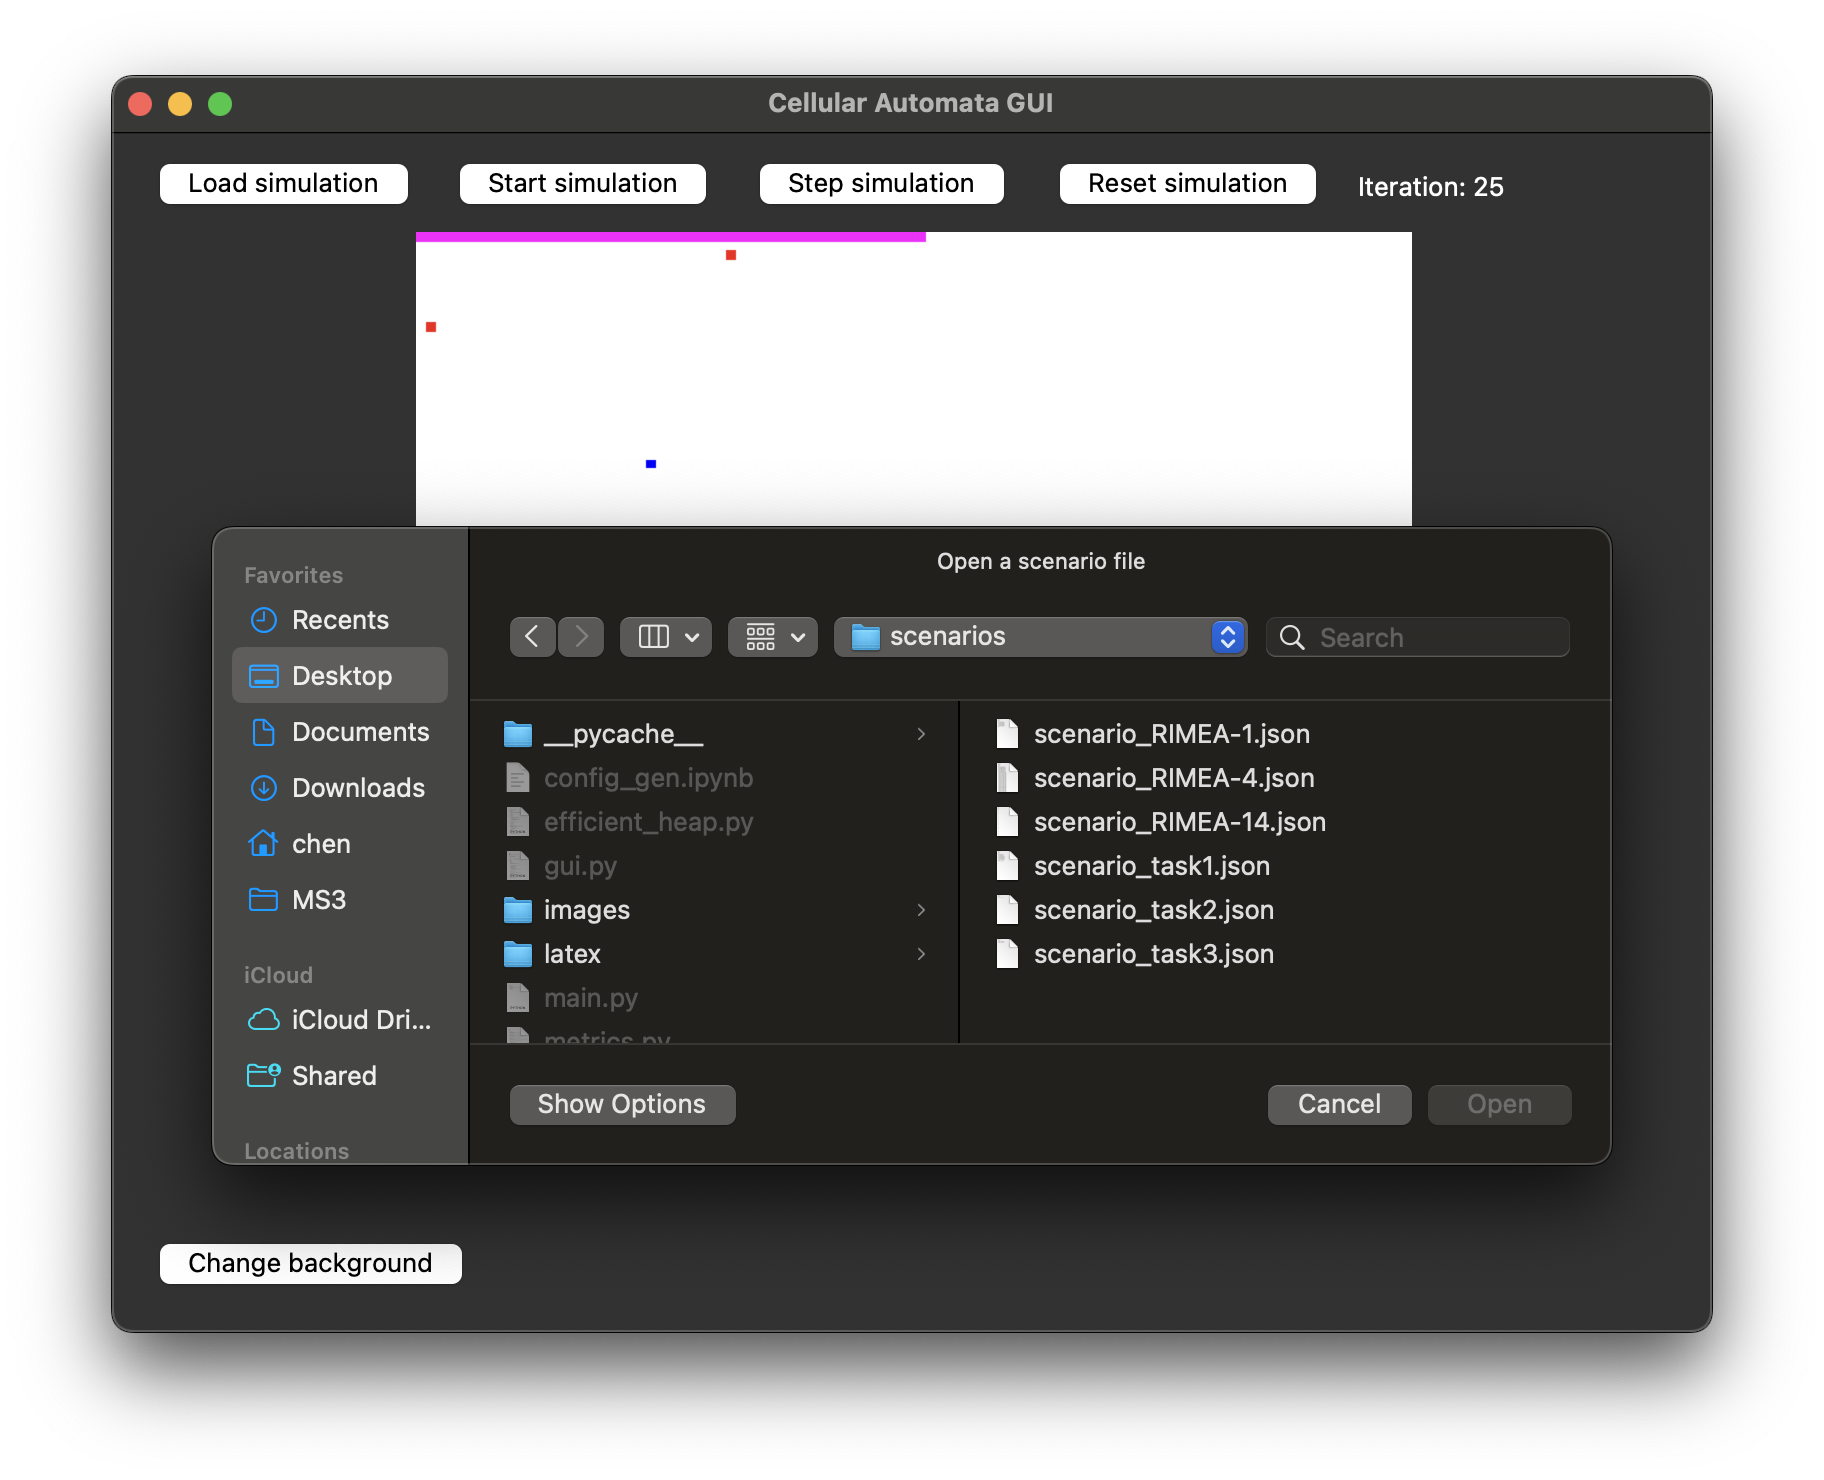
\includegraphics[width=0.4\textwidth]{report-template/image/Task1_1.png}}
\subfigure[Start simulation]{
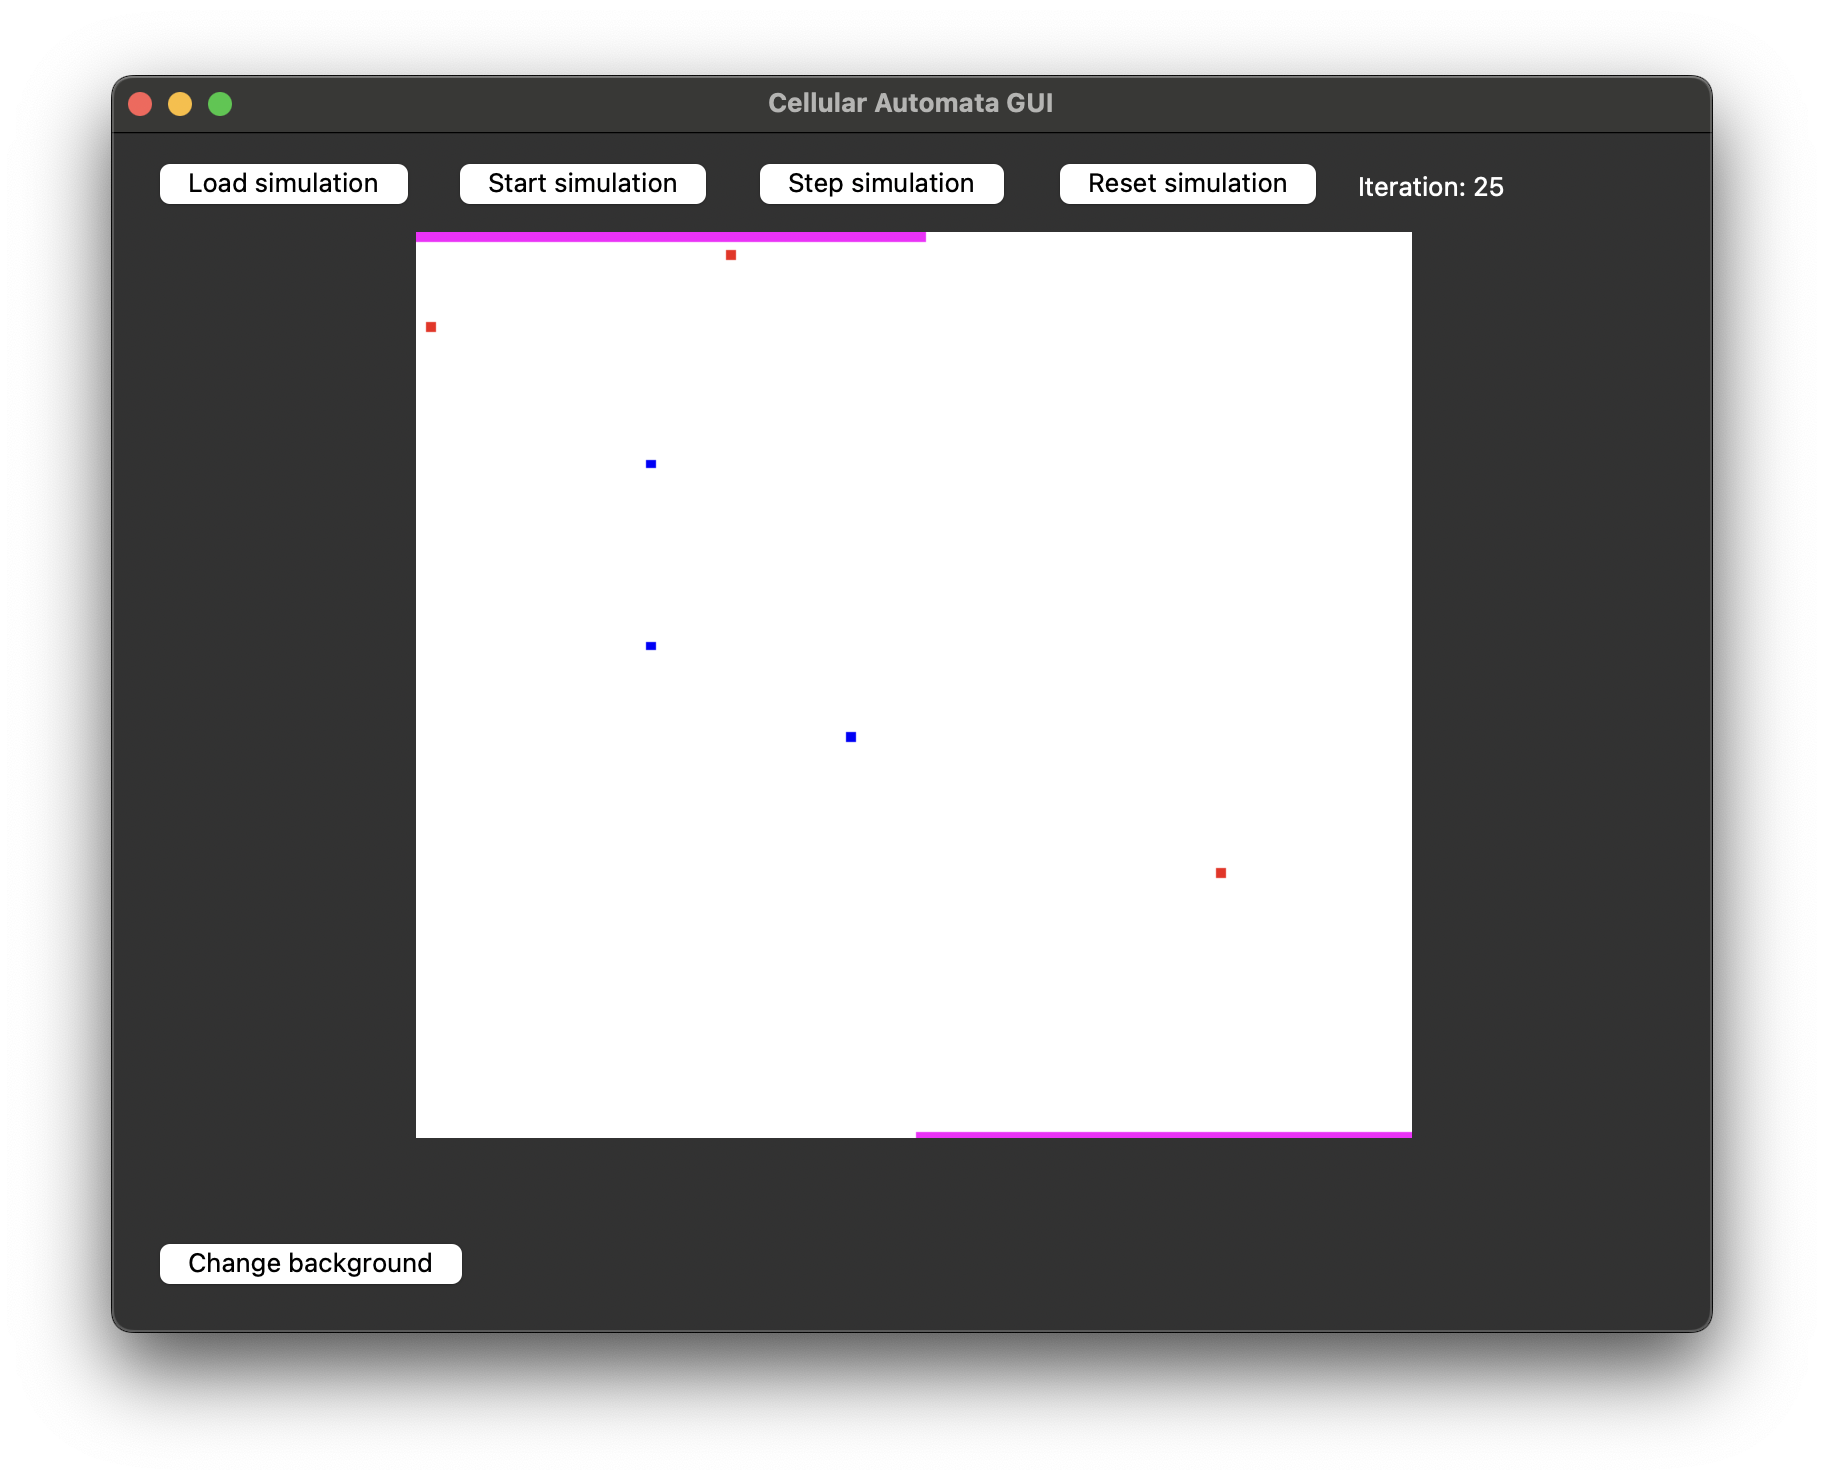
\includegraphics[width=0.4\textwidth]{report-template/image/Task1_2.png}}
\subfigure[Simulation Finished]{
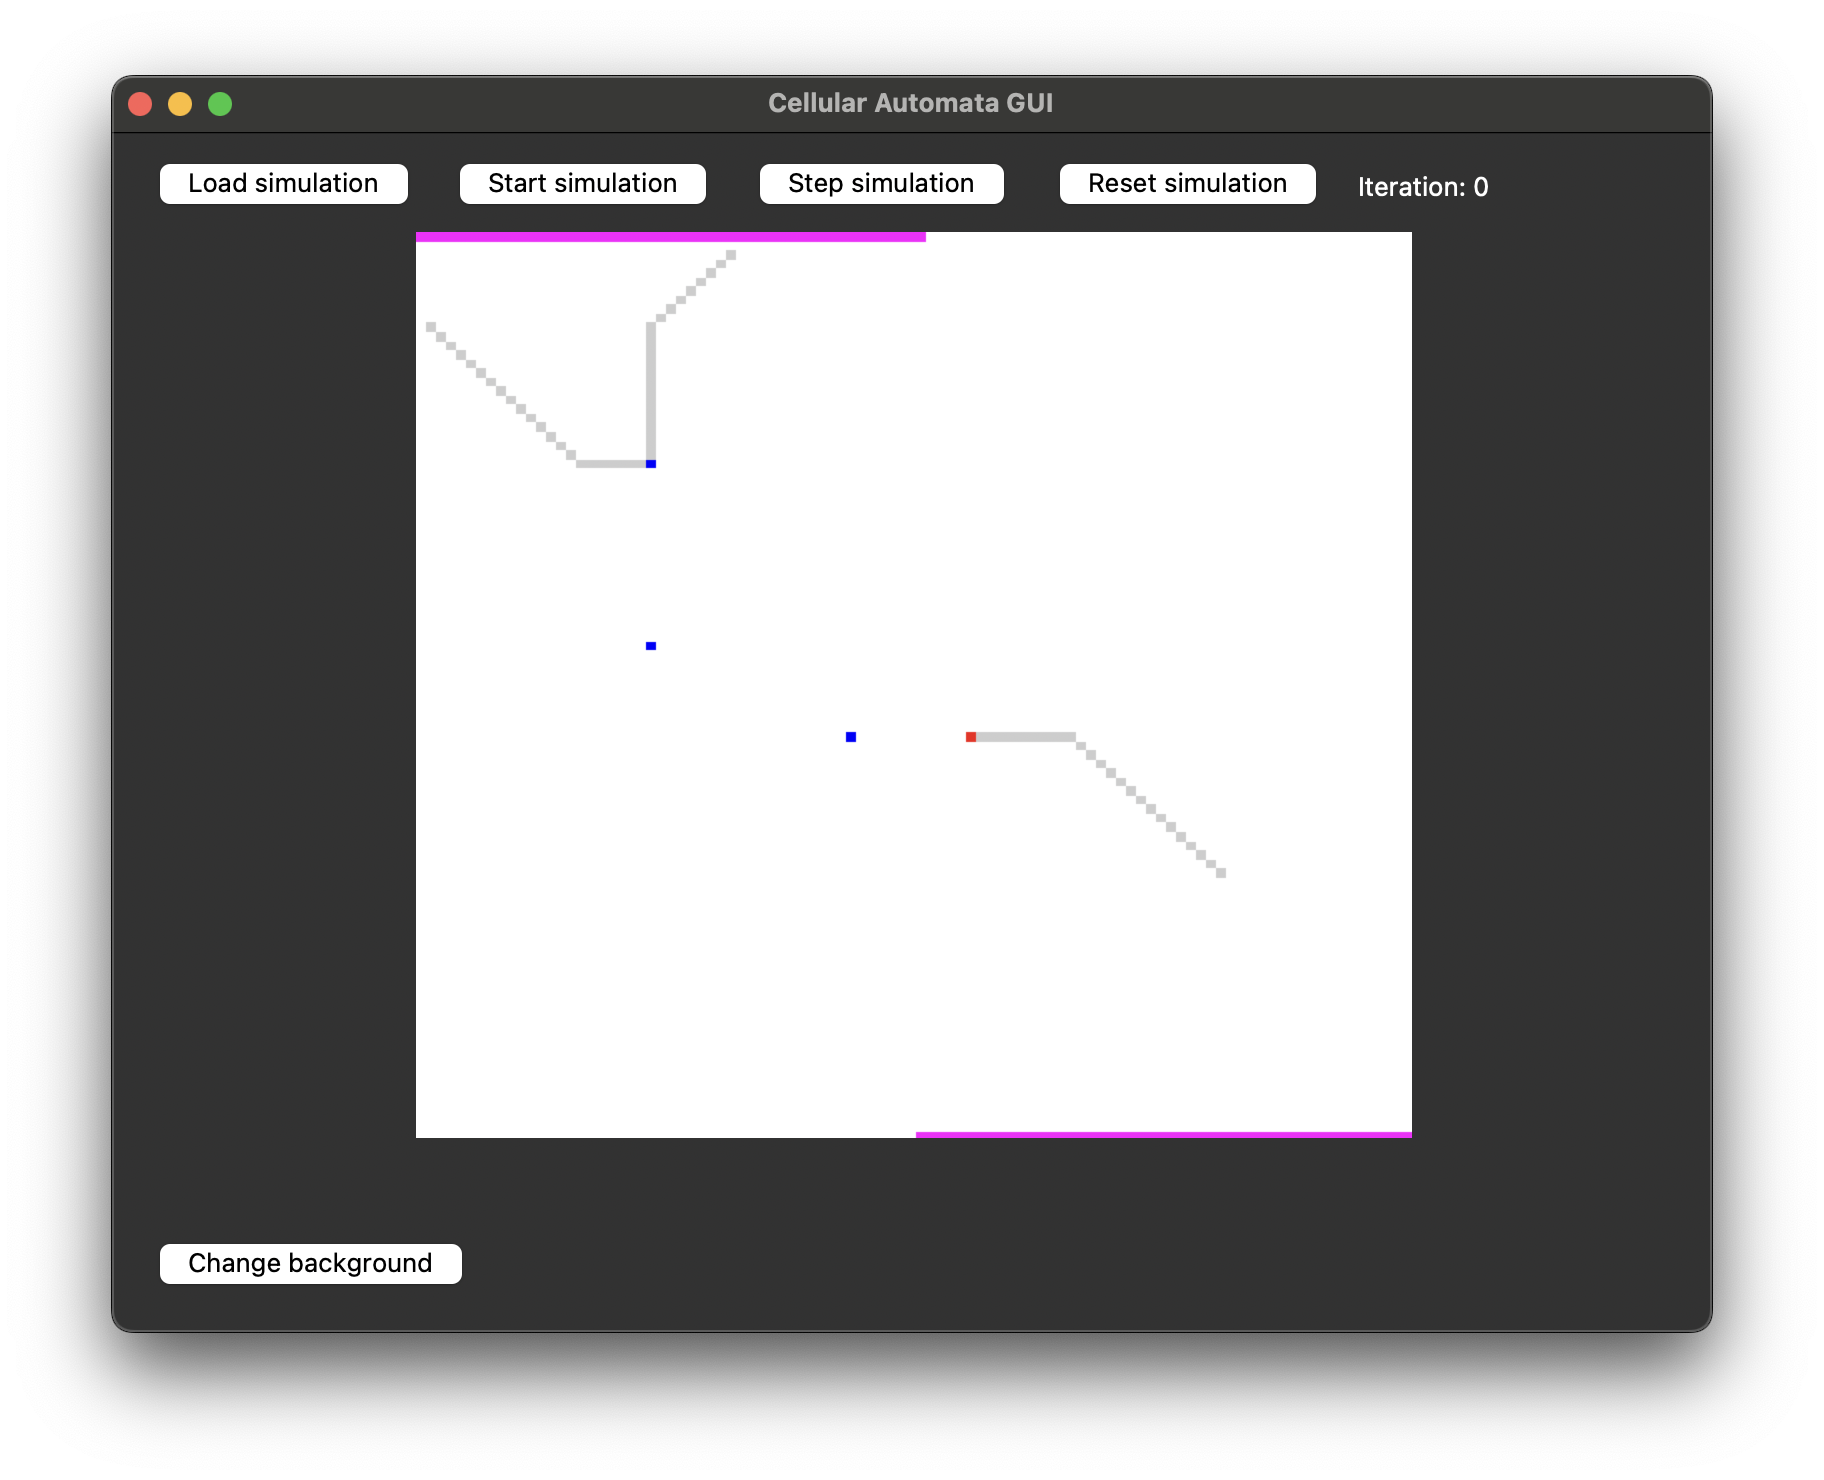
\includegraphics[width=0.4\textwidth]{report-template/image/Task1_3.png}}
\subfigure[Target reached]{
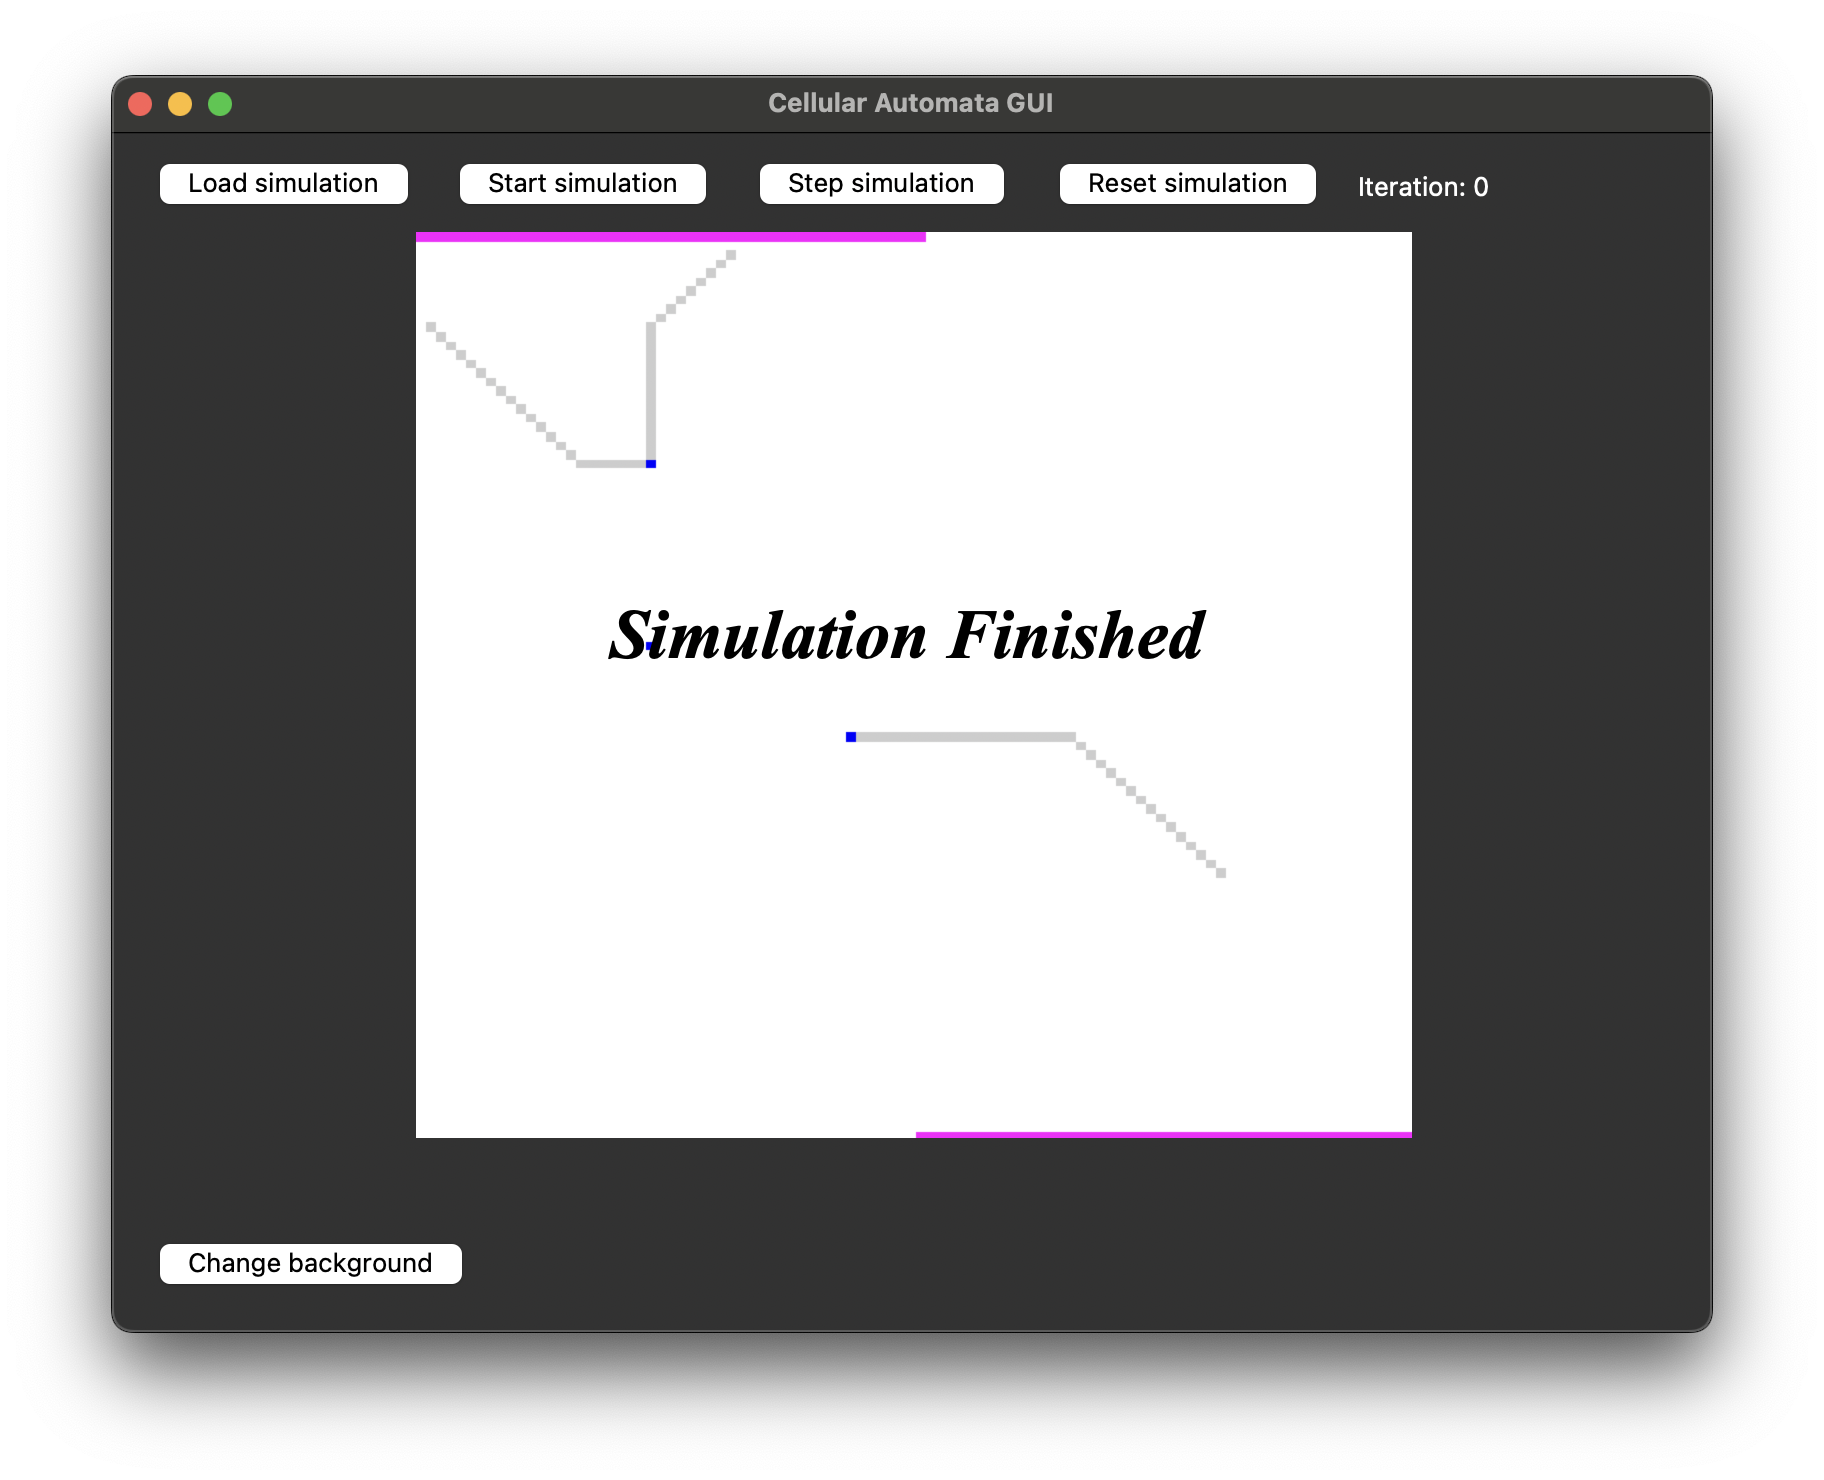
\includegraphics[width=0.4\textwidth]{report-template/image/Task1_4.png}}
\subfigure[Visualizing target distances]{
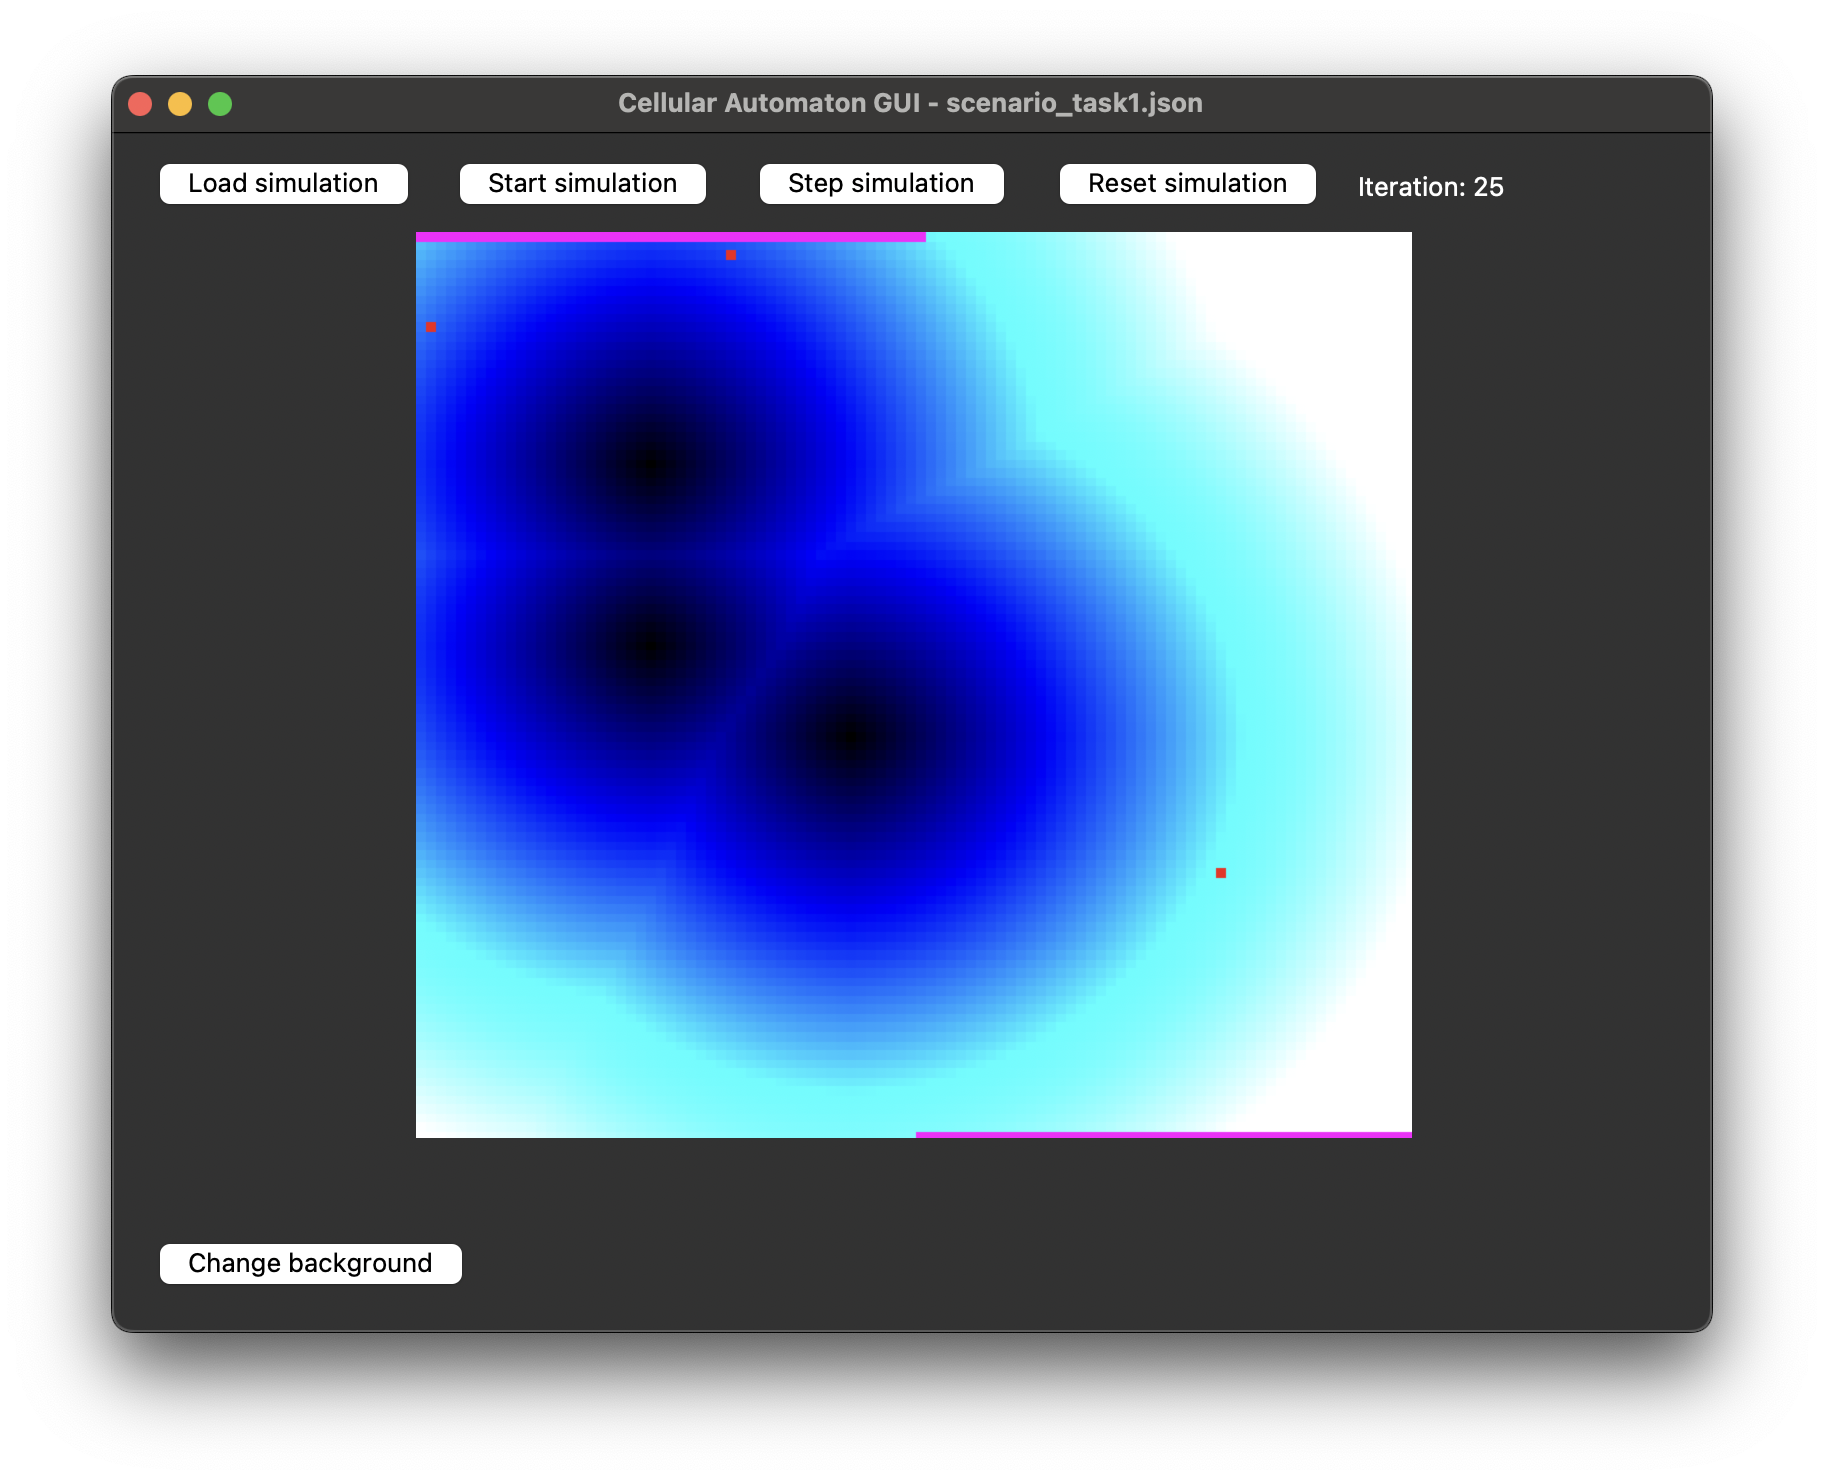
\includegraphics[width=0.4\textwidth]{report-template/image/Task1_5.png}}
\caption{Use of the GUI}
\label{task1}
\end{figure}
\end{task}

\newpage
\begin{task}{2, First step of a single pedestrian}
In the  second task we want to test the basic functionalities of the simulations in a simple scenario. Here we created a new scenario file that satisfies the following  specifications:
\begin{itemize}
    \item Iterations: 25
    \item Cell size: 50x50
    \item Target position: (25, 25)
    \item Pedestrian position: (5, 25)
\end{itemize}
The scenario can be opened via the load simulation button and selecting "scenario\_task2.json" in the dialogue window. To run this test from CLI run the following command:
\begin{verbatim}
python main.py --scenario scenario_task2.json --algorithm S
\end{verbatim}
Afterwards, the simulation finishes with the pedestrian reaching the target and waiting there.
\begin{figure}[H] 
\centering
\subfigure[Initial state]{
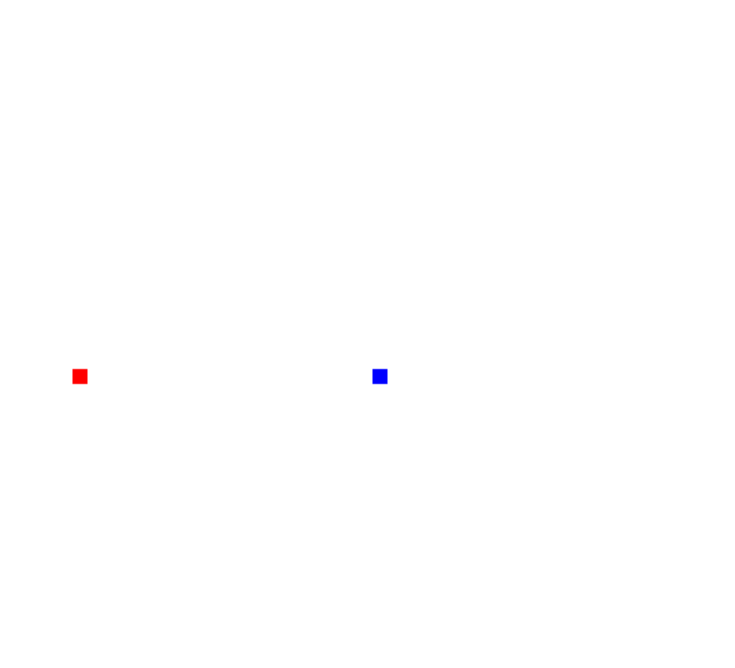
\includegraphics[width=0.4\textwidth]{report-template/image/Task2_1.png}}
\subfigure[Final state]{

\includegraphics[width=0.4\textwidth]{report-template/image/Task2_2.png}}
\caption{Simulation of task 2}
\end{figure}

In the Figure \ref{pedestrian_block} we make certain cells inaccessible by adding a vertical line of obstacles to block the pedestrian. Here we still use the standard movement algorithm with Euclidean distance. We treat all 8 connected neighboring cells as the "next step" to calculate the optimal step. As the pedestrian reached the cell neighbouring to the obstacles, the pedestrian get stuck at that point. Use the following command to reproduce this example.

\begin{verbatim}
python main.py --scenario scenario_task2a.json --algorithm S
\end{verbatim}

\begin{figure}[H] 
\centering
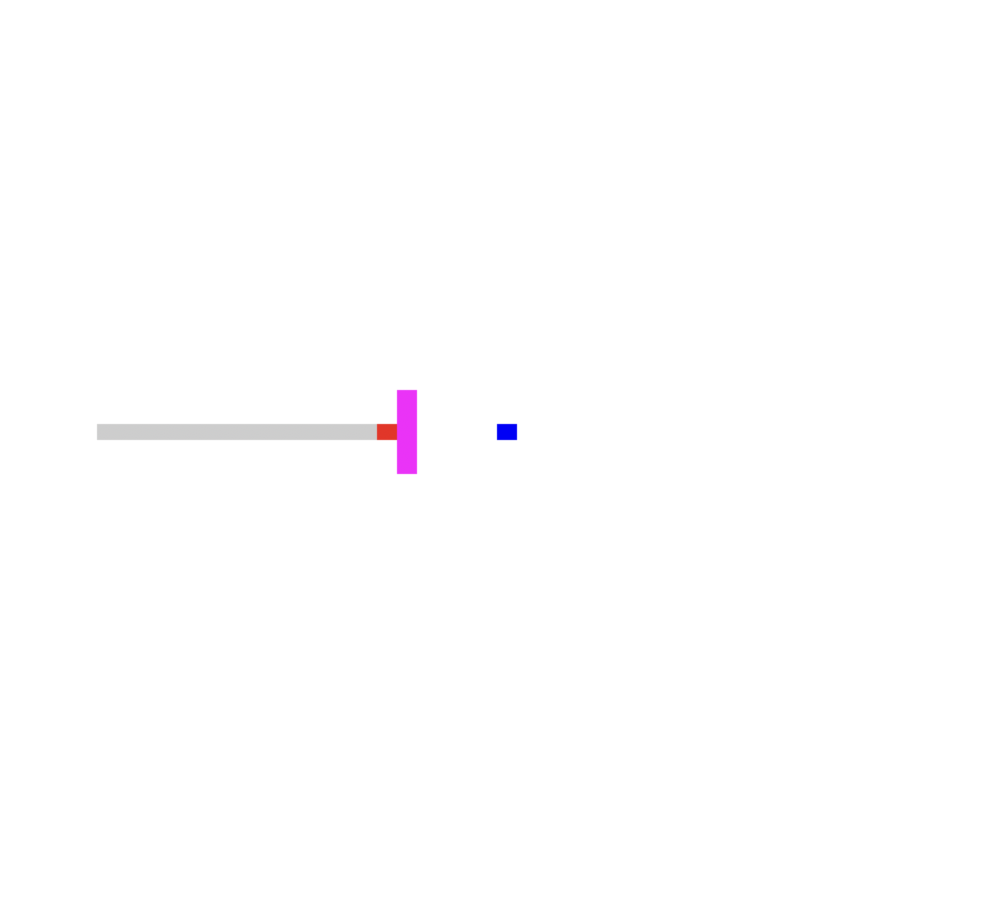
\includegraphics[width=0.4\textwidth]{report-template/image/Task1_7.png}
\caption{Pedestrian blocked by obstacle}
\label{pedestrian_block}
\end{figure}
\end{task}

\begin{task}{3, Interaction of pedestrians}
The third task serves to manage the speeds of pedestrians. To do this, we created a scenario where 5 pedestrians are at approximately the same distance from a target, forming a circle. In particular, as we want to check the difference in speed between horizontal, vertical and diagonal movements. In the scenario there are four pedestrians forming a cross with respect to the centre, providing the horizontal and vertical movements, and we have placed a pedestrian at the same distance on a diagonal.
\begin{figure}[H] 
\centering
\subfigure[Initial state]{
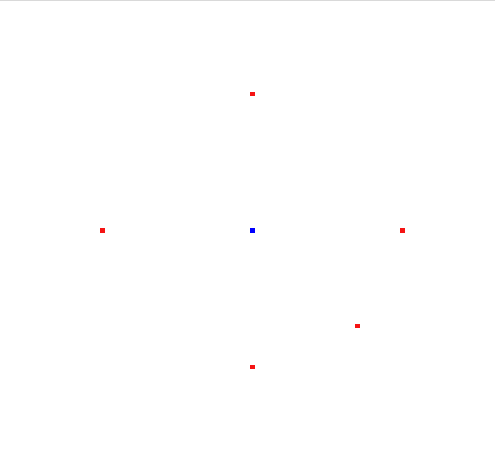
\includegraphics[width=0.45\textwidth]{report-template/image/Task_3_1.png}}
\subfigure[Final state]{
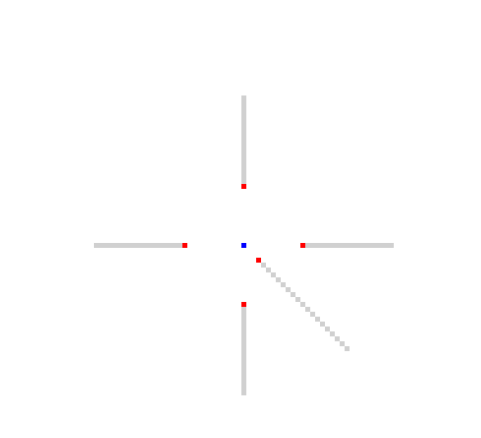
\includegraphics[width=0.45\textwidth]{report-template/image/Task_3_2.png}}
\caption{Initial simulation of task 3}
\label{init_sim_3}
\end{figure}

As we can observe in Figure \ref{init_sim_3}b, the diagonal path to the target is faster than the horizontal and vertical ones. That is because our system is using a discrete grid, but the distance from a pedestrian to the target is computed using the Euclidean distance. Therefore, if a pedestrian moves horizontally or vertically, it is advancing a distance of 1, but if it moves diagonally it is advancing a distance of $\sqrt{2} = 1.41...$, thus travelling more distance in the same time. 

We tried to solve the problem by putting a penalty on the diagonal movement. We calculated the Euclidean distance travelled by a pedestrian and when a series of time steps were fulfilled we calculated its velocity as the radius of the distance and the number of those time steps. If the pedestrian's speed was greater than the desired speed, entered as a parameter in the scenario's .json file, it was forced to stop at the next time step. As we can observe in Figure \ref{sim_task3}a, this method achieved that all pedestrians reached the target at the same time step, reducing the difference in their speeds. However, it is not very realistic for a crowd to be constrained in diagonal motion only, so we generalised this concept and made the motion of pedestrians stochastic, still trying to penalise more the diagonal movements. We achieve this using formula (1):
 \begin{equation}
\frac{\text{desired\_speed}}{\text{dist}(\text{position}, \text{min\_cost\_pos})} < \epsilon
\end{equation}
where \(\epsilon\) is a random number \(\epsilon \in [0,1]\). This formula is checked inside the \texttt{update\_step} function in the Pedestrian class, and if the condition is fulfilled, the pedestrian does not advance a position in that time step. Basically, the pedestrian's speed becomes a probability distribution, since we are comparing the ratio between their desired speed and the Euclidean distance to a random number. 

If the Euclidean distance from the pedestrian's current position and its next position is greater (it is diagonal) it is more likely to stop than making a horizontal or vertical movement. On the other hand, as the divisor is the desired velocity, if this is very large, it will be less likely to stop as well. Therefore, in this simple way a velocity distribution can be modelled for the pedestrians with the diagonal motion constraints.

In Figure \ref{sim_task3}b we can observe a non-uniform speed distribution allowing horizontal and vertical paths to be equally fast as diagonal ones. In Figure \ref{sim_task3}c is shown the comparison between the desired speed and the actual speed of each of the pedestrians. The stochastic distribution of speeds can be noticed. For example the 3 fastest pedestrians in Figure \ref{sim_task3}b have a higher current speed and are at the top of the graph, and the last two pedestrians have a current speed of approximately 0.1 less.
\begin{figure}[H] 
\centering
\subfigure[First implementation]{
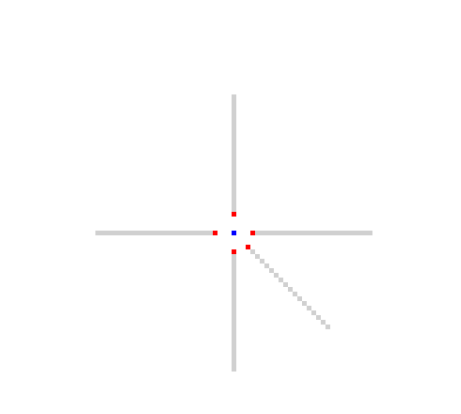
\includegraphics[width=0.4\textwidth]{report-template/image/Task_3_3.png}}
\subfigure[Stochastic implementation]{
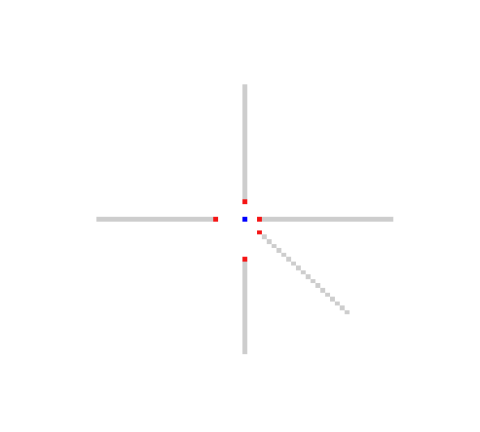
\includegraphics[width=0.4\textwidth]{report-template/image/Task_3_4.png}}
\subfigure[Actual speed vs desired speed distribution]{
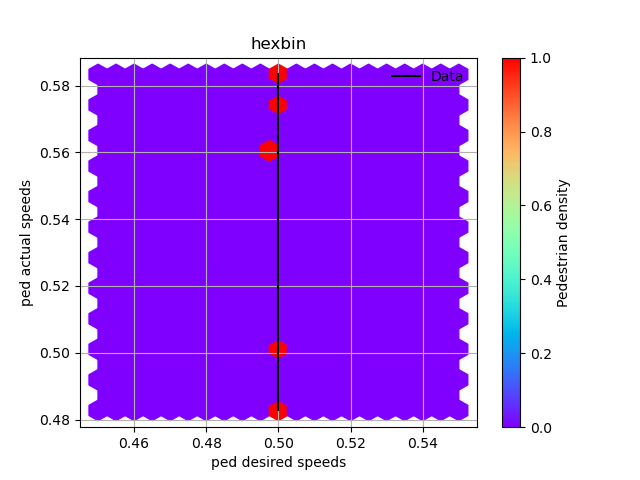
\includegraphics[width=0.4\textwidth]{report-template/image/plot_task3.png}}
\caption{Implementations of task 3}
\label{sim_task3}
\end{figure}

Pedestrian avoidance was not needed for this exercise, however it is still a feature of pedestrian interaction. Pedestrian avoidance is explained in the next section.
Use the following command to run the experiment:
\begin{verbatim}
python main.py --scenario scenario_task3.json --algorithm S 
\end{verbatim}
\end{task}

\begin{task}{4, Integrating a new model}

\paragraph{1. Implementation of the SIR Model into Vadere}

\begin{figure}[H]
\centering
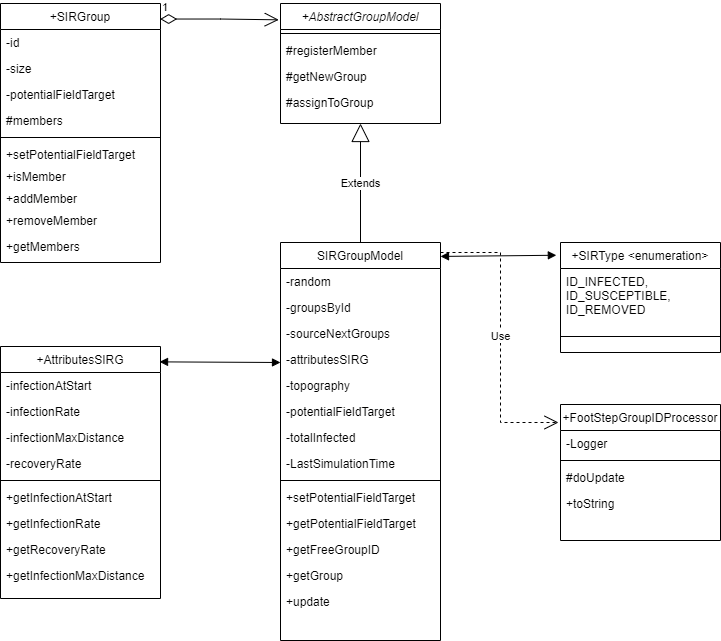
\includegraphics[width=0.7\textwidth]{report-template/images/taask4.1.png}
\caption{UML diagram of SIR Model}
\label{fig:fig4uml}
\end{figure}
The UML diagram above \ref{fig:fig4uml} describes the relationships between the classes \verb+SIRGroupModel+, \verb+SIRGroup+, \verb+AbstractGroupModel+, \verb+AttributeSIRG+, \verb+SIRType+ and \verb+FootStepGroupIDProcessor+. For some classes only important functions were listed.
\begin{description}
    \item \verb+SIRGroupModel+ is the main class for handling the behaviour of groups in the SIR model. It keeps track of the group ids and assigns pedestrian to each of the groups in the SIR model. The update function does most of this work. It implements calculation for infecting and recovering pedestrians and also contains the efficient neighbourhood lookup using LinkedCellsGrid to check for susceptible pedestrians.
    \item \verb+SIRGroup+ contains essential information about a SIR group as well as adding and removing members. Furthermore it defines the type of the generic class \verb+AbstractGroupModel+, which \verb+SIRGroupModel+ inherits from. This leads \verb+SIRGroupModel+ returning groups of type \verb+SIRGroup+ for the inherited functions. 
    \item \verb+AttributesSIRG+ contains the parameters of our SIR model and is saved as attribute in the \verb+SIRGroupModel+. Infection rate and recovery rate can be changed here for example. Additionally the values in this class the initial parameters when loading the SIR model into Vadere and can be changed in the Vadere editor before running a simulation.
    \item \verb+SIRType+ is simple enumeration class which contains 3 different states in the SIR model. This class is used in \verb+SIRGroupModel+ to determine the pedestrian state in the SIR model.
    \item \verb+FootStepProcessor+ uses \verb+SIRGroupModel+ to log information about SIR simulation. This class is an additional output processor that can be linked in the Vadere. When running the SIR model this processor output additional information about the SIR model.
\end{description}

% uml
%\textbf{SirGroupModel}: is the main class which is the extension of the AbstractGroupModel. 
%Group the pedestrains by the ID, and also updating method does the main job of traversing all the pedestrians, checking the infected rate, and determining if the pedestrian is lucky enough to get infected or not. 
%\textbf{SIRgroup}: this class is the aggregation of the AbstractGroupModel, a unique ID for every member, which can be used to manipulate the members to be added, or deleted. 
%\textbf{AttributeSIRG}:  associated with the  SirGroupModel, contains the basic information of infection state, infection rate, and Recovery rate, and the infection maximal distance. 
%\textbf{SIRType} also associated with the SIRgroupModel, store the states of the pedestrian.  \textbf{FootStepGroupIDProcessor} one additional class used by the SirGroupModel, outputs the processor and saves the result as a file. the doUpdate method is the most important, every step will update new info on the current time step, pedestrian, and group. 

\paragraph{2. Description of the output processor}
In this part we use our own output processor \verb+SecondGroupIDProcessor+ instead of \verb+FootStepGroupIDProcessor+, which can be found in the same folder as the other output processors. This class simply writes down at each time-step the pedestrian id and group id of the pedestrian. This way even pedestrians that did not move are tracked unlike in the footstep processor and this allows for a more direct output. Of course we could have set up a program to read the footstep processor output and memorize the group ID from the previous time-step if the next time-step does not include a pedestrian but this did not occur to us at the time.

In the visualization we use a python notebook that loads the file and extracts the group IDs in each time-step and then plots percentages of the group IDs. This is handled in the python notebook \verb+visualizeSIR.ipynb+ which generates graphs tracking changes of the SIR groups. \textit{Note that for task 4 and task 5 the vadere project with its scenarios are placed in the folder} \verb+Exercise-2\vadere-project-tas45+.

\paragraph{3. SIR group visualization}
To color the pedestrians based on their group we need to put the group id and its corresponding color into the \verb+colorMap+ in the class \verb+SimulationModel.java+. We assigned the following colors to each group id:
\begin{itemize}
    \item 0 = Red
    \item 1 = Black
    \item 2 = Blue
\end{itemize}
We also didn't use green or white for susceptible individuals, because the pedestrian spawning area is visualized with green and the background color is white. To visualize the pedestrians according to group color during simulation we need to set the \verb+DefaultSimulationConfig.agentColoring = AgentColoring.GROUP+. It is noteworthy that due to our own implementation of the output processor in \verb+SecondGroupIDProcessor+ we have only implemented the visualization of groups during simulation. Visualization of groups in post-visualization is not supported in this iteration of our code.

\paragraph{4. Using LinkedCellsGrid to improve efficiency} To increase the efficiency of finding nearby pedestrians we modified the \verb+update(...)+ function in \verb+SIRGroupModel.java+. To get the neighbourhood of given radius more efficiently the LinkedCellsGrid slices the 2 dimensional space into uniform squares of given side length. It then only checks the squares which are less than the radius of the neighbourhood away from a given position's square.

\paragraph{5.1 Test: comparing infection rates}
% Tested+visualized scenario in figure 6, left, without recovered state?
% How long does it take for half of the population to be infected?
% Increase the infectionRate of the model using the GUI, and run the previous test again. Plot both results in one graph. How long does it take to infect half the population now?
In this test we setup a large area in which we randomly placed a 1000 pedestrians uniformly distributed. In this test we want to compare how fast 50\% of the pedestrians become infected depending on the infection rates. We have setup the same starting amount of $10$ infected pedestrians in both scenarios. In this test we only changed \verb+infectionRate+, but a full list will be provided at the end of this section. Running the tests yields the following results, where the \verb+infectionRate+ is the probability for and the time is how long it takes until 50\% of the pedestrians are infected:
\begin{center}
\begin{tabular}{ |c|c|c| } 
 \hline
& Scenario (a) & Scenario (b) \\
\hline
\verb+infectionRate+ & $0.01$ & $0.05$ \\
\hline
time (in seconds) & $36.2$ & $4$\\
\hline
\end{tabular}
\end{center}
We see that with $5$ times the infection rate the time until 50\% of the pedestrians are infected decreases from $36.2$ seconds to $4$ seconds. We know from the mathematical nature of infection spreading that it has an exponential behaviour. Hence the immense decrease in time until 50\% is infected is expected. In the figures \ref{fig:fig6sim} below we see the results after running both simulations. Further more in figure \ref{fig:fig6sim}(c) we see a graph comparing the infection spread between both scenarios.
\begin{figure}[H]
\centering
\subfigure[infection rate 0.01 at second 36.2]{
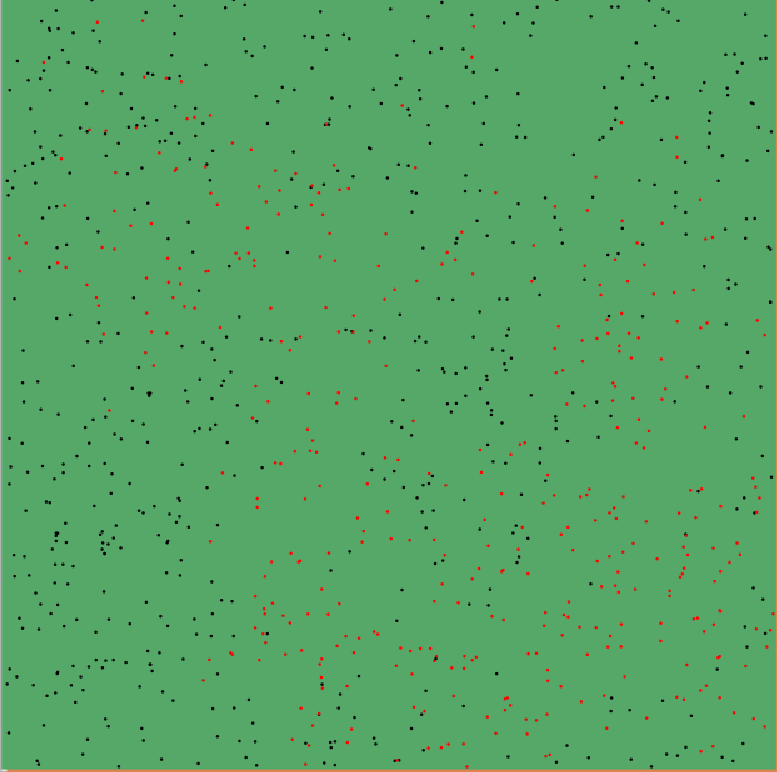
\includegraphics[width=0.4\textwidth]{report-template/images/001_no_recovery_16_2.png}}
\subfigure[infection rate 0.05 at second 4]{
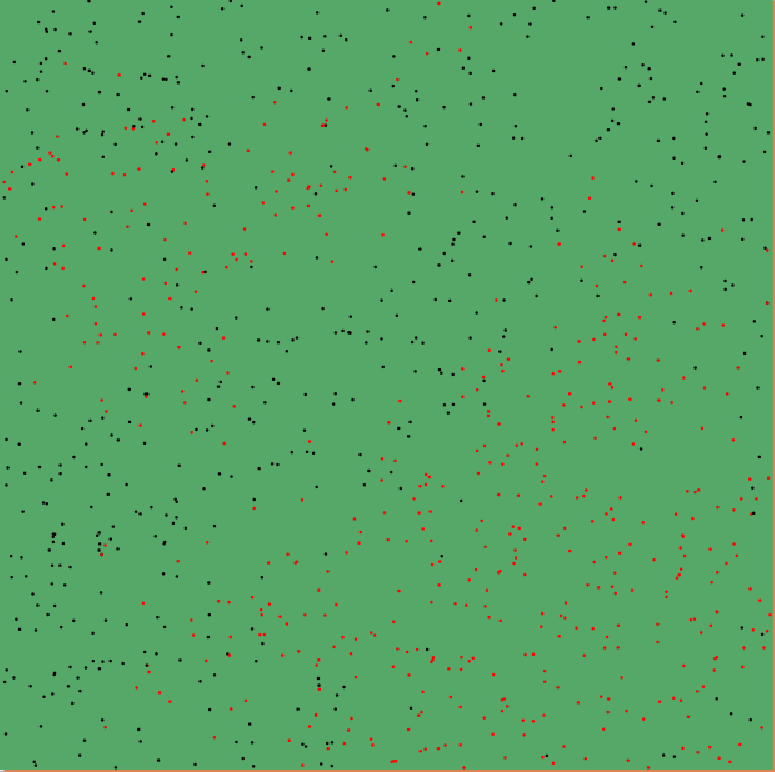
\includegraphics[width=0.4\textwidth]{report-template/images/005_no_recovery_4_0.png}}
\subfigure[Comparison between different spread rates]{
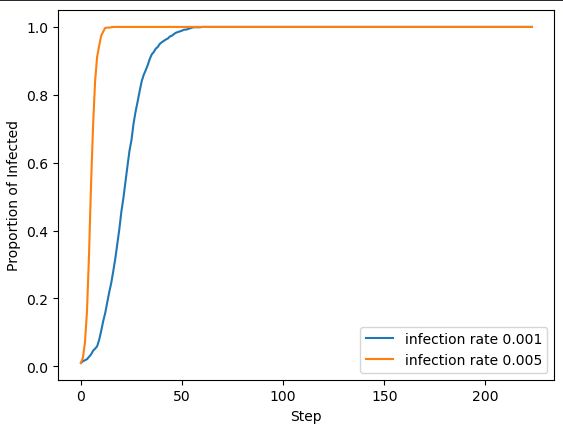
\includegraphics[width=0.5\textwidth]{report-template/images/rateplot.png}}
\caption{Comparison of the figure 6 simulations}
\label{fig:fig6sim}
\end{figure}

\noindent Scenario \ref{fig:fig6sim}(a) parameters
\begin{verbatim}
"infectionsAtStart" : 10,
"infectionRate" : 0.01,
"infectionMaxDistance" : 10.0,
"recoveryRate" : 0.0
"infectionRateWhenAdded" : 0.0
\end{verbatim}
Scenario \ref{fig:fig6sim}(b) parameters
\begin{verbatim}
"infectionsAtStart" : 10,
"infectionRate" : 0.05,
"infectionMaxDistance" : 10.0,
"recoveryRate" : 0.0
"infectionRateWhenAdded" : 0.0
\end{verbatim}

\paragraph{5.2 Test scenario corridor with counterflow}
% New scenario: corridor. How many pedestrians get infected in counterflow?

In this test we have two groups of 100 pedestrians walking in opposing directions in a corridor of 40x20 meters size. The pedestrians are released over time. One of the groups has 10 infected pedestrians. We now  want to know how much infection spreads given that one group has no infected pedestrians.

At first we ran the simulation with the infection rate set to 0.001 (1.0E-3) and the absorbers enabled, this did not allow for the pedestrian infection counts to be reliably counted and the infection spread even after the groups passed each other. We could have written some code to allow for getting the numbers of infected in each group from the resulting file and either extrapolating the number of pedestrians infected during inter-group contact or changed to code to allow for the groups to be set separate. Instead we first tried to achieve this with the tools at hand.

To minimize infection between group members and make the calculation easier we simply set the infection rate really low to 0.0001 (1.0E-4) and run the simulation with the target absorbers disabled. Observing the image we can easily count that two pedestrians got infected. From before in the simulation we can see that no infections between group members in the group originally without infected occurred before that point.

\begin{center}
\begin{tabular}{ |c|c|c| } 
 \hline
& Corridor (a) & Corridor (b) \\
\hline
\verb+infectionRate+ & $1.0E-3$ & $1.0E-4$ \\
\hline
\end{tabular}
\end{center}
\begin{figure}[H]
\centering
\subfigure[infection rate 0.001 at second 20]{
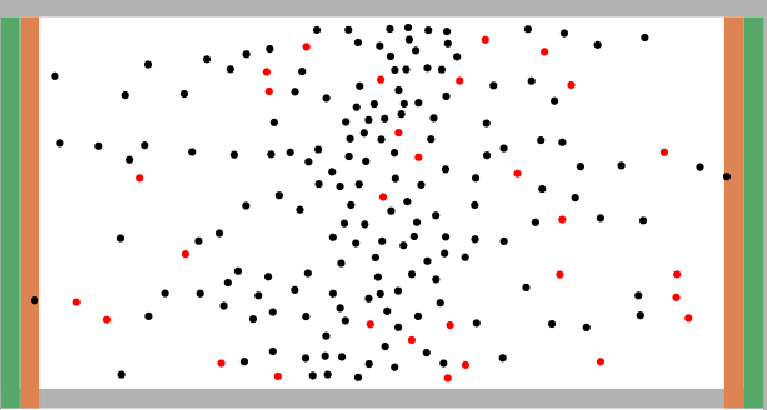
\includegraphics[width=0.4\textwidth]{report-template/images/corridor_20_0.png}}
\subfigure[infection rate 0.0001 after meet]{
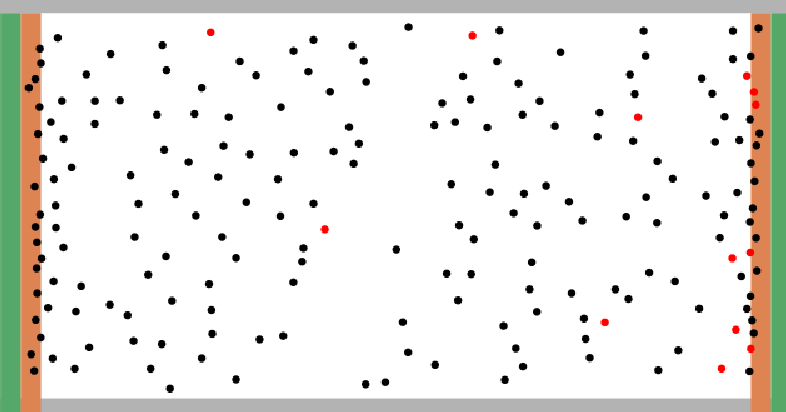
\includegraphics[width=0.4\textwidth]{report-template/images/0001_corridor_after_meet.png}}
\subfigure[infection rate 0.0001 at the end]{
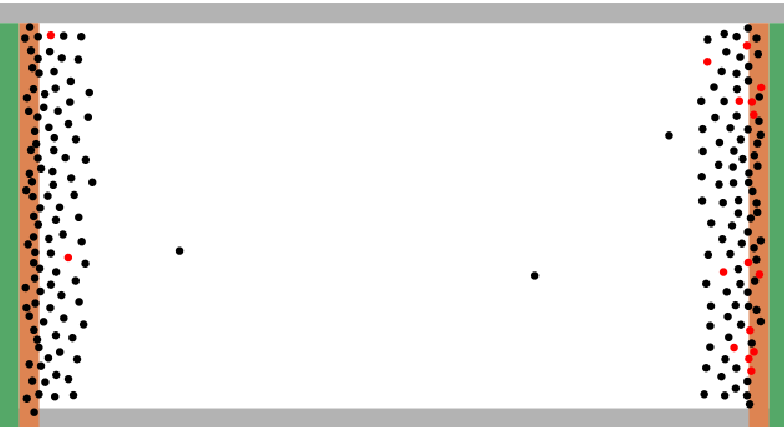
\includegraphics[width=0.4\textwidth]{report-template/images/0001_corridor_end.png}}
\caption{The corridor scenario}
\label{fig:corridor}
\end{figure}

\noindent Scenario \ref{fig:corridor}(a) parameters
\begin{verbatim}
"infectionsAtStart" : 10,
"infectionRate" : 1.0E-3,
"infectionMaxDistance" : 10.0,
"recoveryRate" : 0.0
"infectionRateWhenAdded" : 0.0
\end{verbatim}
Scenario \ref{fig:corridor}(b)(c) parameters
\begin{verbatim}
"infectionsAtStart" : 10,
"infectionRate" : 1.0E-4,
"infectionMaxDistance" : 10.0,
"recoveryRate" : 0.0
"infectionRateWhenAdded" : 0.0
\end{verbatim}


\paragraph{6. Decoupling infection rate from simulation time-step}
To do this we initially assume that an infected pedestrian has a chance of $(1-p)$ to not spread the disease. Let the probability of an infected pedestrian not spreading the disease at a \textit{single} time-step be $(1-q)$. Let $n$ be the amount of time-steps in a second, we then have the following equation:
\begin{align}
    (1-q)^n &=(1-p)\\
    (1-q) &= (1-p)^{1/n}
\end{align}
Note that the amount of time-steps $n$ in a second is equivalent to $n = 1/t$, where $t$ is the delta time or time since the last time-step has happened. Inserting this gives us the following:
\begin{align}
    (1-q) &= (1-p)^{1/(1/t)}\\
    (1-q) &= (1-p)^t
\end{align}
We have shown that that if a pedestrian does not spread the disease with probability $1-p$ every second, the chance to not spread the disease in delta time $t$ is $(1-q) = (1-p)^t$. Hence the chance that a pedestrian does spread the infection at a time-step is simply $1-(1-p)^t$.

To implement this we added an attribute \verb+LastSimulationTime+ to \verb+SIRGroupModel.java+, which is used to calculate the delta time $t$. In the \verb+update(...)+ function of the same class we then use the expression $1-(1-p)^t$ to correctly calculate the probability of infecting a pedestrian. Note that the same formula is used for recovery as well (See task 5.2).

The simulation rate still technically affects the infection. The infection radius and infection ticks caused by the new infected could be taken into account. For example if we instead simulated the infection retroactively. This however would necessitate ignoring simulation rate to an extent and therefore seems like a sub-optimal solution. If we truly wanted to allow the user to remove this inaccuracy at the cost of processing power it could be possible to add a separate simulation rate setting for the infection spread.



\paragraph{7. Possible extensions}
So far the integrated SIR model only contains basic features to model the spread of infections. Including the implementation from Task 5 the model would additionally consider the recovery of people. Still the SIR model as presented in \cite{boccara2010model} considers removed people instead of recovered people and therefore we only model infection in a simplified manner. In the following we will discuss possible extensions to improve the model.

The first possible extension is allowing recovered people to infect susceptible people. Recovered people realistically can still carry the infection around for a certain time. Therefore recovered people would still be able to infect susceptible people.

The second possible extensions is allowing recovered people to become reinfected. Simply speaking an infection could mutate within a group of people after a certain time frame. This mutated infection would then also be able to spread to recovered people and reinfect them.

Further more on completing the SIR model, under removed individuals we can consider subgroups other than recovered people. Here for example we could add deceased, permanently immune and/or isolated individuals. Disregarding the realism for a moment in the Vadere simulation this would mean deceased pedestrians could be modeled as static pedestrians. Permanently immune individuals would have 0 chance of being reinfected, where as isolated individuals are modeled as pedestrians performing social distancing.

At this point it becomes clear that the SIR model considers infection from a very general standpoint with the least amount of assumptions about the diverse factors that play a role in reality. The SIR model implemented in Vadere assumes that infections are spread by being in the vicinity of an infected pedestrian. This assumes that infections are spread through human interaction only. In Vadere we can extend this implementation to contain other groups that are carriers of infections. For example certain pedestrians could  be representing animals or insects. Similarly an infection that spreads through the air would could also be modeled as a group of infected pedestrians.

Beyond the assumption of modeling infections spreading in large crowds, we can also imitate the spread within social structures in Vadere. As shown in \cite{wolfram2020} an agent-based network provides an abstraction to model social connections. A majority pf people don't spend their time in crowds, but in certain environments with a set of other people e.g. workplace, school, university. This could be imitated in Vadere to a decently realistic degree. For example we can have the pedestrians form multiple smaller crowds at a sequence of targets and remain there for a certain time span. Here the targets can represent a home, workplace, school, supermarket, etc. A potential issue in this model would lie within the movement of the pedestrians between the targets. While infections do occur when traveling between different locations, this proposed model does not explicitly capture infections during traversal.

Overall we conclude this discussion with the fact that spread of infections in reality are very difficult to model due to a variety of factors. Every model is only an approximation of reality and depending on the assumptions made in the model, they provide a decently accurate depiction on certain aspects of it.

\end{task}
\newpage
\begin{task}{5, Bifurcations in crowd dynamics}
In this task we want to apply our knowledge about bifurcation theory to analyze and describe a given SIR model from \cite{shan2014bifurcations}. Unless mentioned all tests were performed with the following values:
\begin{align*}
    A = 20,
    d = 0.1,
    \nu = 1,
    \mu_0 = 10,
    \mu_1 = 10.45,
    \beta = 11.5,
    b = 0.022
\end{align*}

\paragraph{Task 5.1: Setup description}
For this task \verb|sir_model.py| and \verb|sir_bed_model_unfinished.ipynb| were used as code framework. Apart from adding the needed documentation we decided to put the plotting from the python notebook into separate functions. These functions can be found in \verb|sir_model_visualization.py|. This makes the code more readable and modular for later use when creating multiple plots of the SIR simulation.

\paragraph{Task 5.2: Model implementation}
Due to moving the plotting functions into a separate python file, the imports were moved as well. The python notebook only needs to import \verb|sir_model_visualization|.

The differential equation based model from \cite{shan2014bifurcations} was implemented according to the exercise sheet in the \verb|model(...)| function in \verb|sir_model.py|.

\paragraph{Task 5.3: Experiments}
In this task we are observing multiple graphs of the SIR simulation as well as its trajectories. For readability we only use a selected choice of plots, but a more extensive collection can be found in the python notebook \verb|sir_bed_model-t5_3.ipynb|. For this we used different initial values $(S_0, I_0, R_0 )$ for the simulation. Here the $S_0$ is the amount of susceptible, $I_0$ the amount of infected and $R_0$ the amount of removed people at $t=0$. We tested with the following initial values.

\begin{align*}
    (195.3,0.052,4.4), (195.7, 0.03, 3.92), (193, 0.08, 6.21)
\end{align*}

We then observed the graphs for a diverse range of the variable $b$, which is the number of hospital beds per 10,000 persons \cite{shan2014bifurcations}. We performed observations for $b\in\{ 0.01, 0.03\}$ in increments of $0.001$. By doing this we can observe a special kind of bifurcation.

In figure \ref{fig:t5_3-trajB} we present a selected choice of the trajectories plotted in 3 dimensions. Here opaque plot lines in red were added. In figure \ref{fig:t5_3-trajB}(b) for $b=0.022$ we can observe a bifurcation. This is indicated by figure \ref{fig:t5_3-trajB}(a) and \ref{fig:t5_3-trajB}(c), where we observe the trajectories before and after this critical point and see 2 different trajectories for the systems stability. Corresponding to the trajectory for $b=0.022$ we see in figure \ref{fig:t5_3-trajB}(d) further plots.

The first plot in \ref{fig:t5_3-trajB}(d) plots the $S,I,R$ counts over time $t$. We can observe a periodic behaviour for these $S,I,R$ counts over time. For $b=0.020$ we would observe a high amplitude at $t=0$ which decays over time. For $b=0.024$ we observe the opposite case with a small amplitude at $t=0$ which grows larger over time. For border cases with $b=0.01$ or $b=0.03$ we observe the periodic behaviour practically vanishing from the graph.

In the second plot of \ref{fig:t5_3-trajB}(d) we show recovery rate and infected counts plotted over time. Similar to the first plot we observe the same periodic behaviour. It is noteworthy that for $b=0.22$ we have seemingly a stable state where the plotted graphs behave like a periodic functions. Unlike this for $b\neq 0.022$ the graphs instead reach a constant value over time $t$.

The last plot in figure \ref{fig:t5_3-trajB}(d) shows the indicator function $h(I)$. As described in \cite{shan2014bifurcations} section 4.2 essentially $h(I)=0$ is a necessary condition for a Hopf bifurcation. We can observe $h(I)=0$ at two points. This functions is defined as
\begin{align*}
    c_0 &= b^2dA\\
    c_1 &= b((\mu_0 -\mu_1 +2d)A + (\beta -\nu )bd)\\
    c_2 &= (\mu_1 -\mu_0)b\nu + 2bd(\beta-\nu)+dA\\
    c_3 &= d(\beta -\nu )\\
    h(I) &= c_0 + c_1 I + c_2 I^2 + c_3 I^3
\end{align*}

In figure \ref{fig:t5_3-sims}(a) and (b) we see the trajectories of for the initial values $(S_0, I_0, R_0 )=(195.7, 0.03, 3.92)$ and $(S_0, I_0, R_0 )=(193, 0.08, 6.21)$ at $b=0.022$. Their corresponding graphs are also showing the periodic behaviour we have observed in figure \ref{fig:t5_3-trajB}(d). We observe that for different starting values  $(S_0, I_0, R_0 )$ the trajectories take a different form. Similar to the Hopf bifurcation in \ref{fig:t5_3-trajB}(b) we see blue and red dots in figures \ref{fig:t5_3-sims}(a) and (b).

\begin{figure}[H]
\centering
\subfigure[$b=0.020$]{
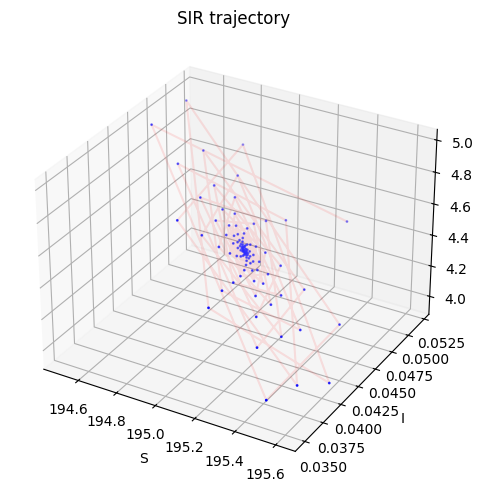
\includegraphics[width=0.3\textwidth]{images/t5_3-traj20.png}}
%\subfigure[$b=0.020$]{
%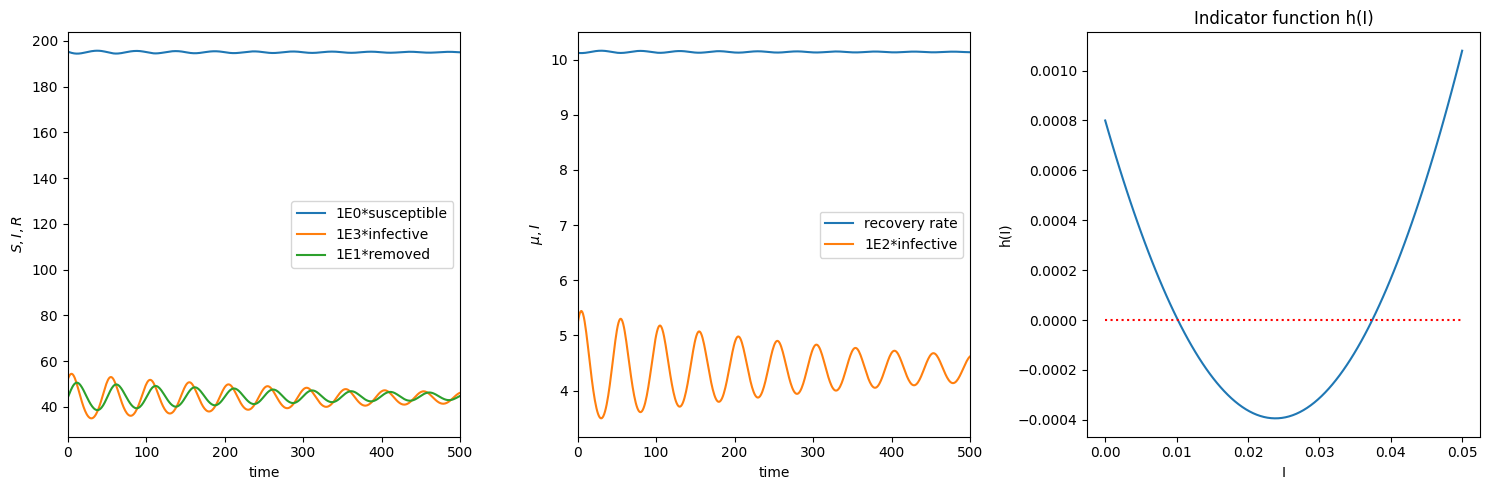
\includegraphics[width=0.6\textwidth]{images/t5_3-sim20.png}}
\subfigure[$b=0.022$]{
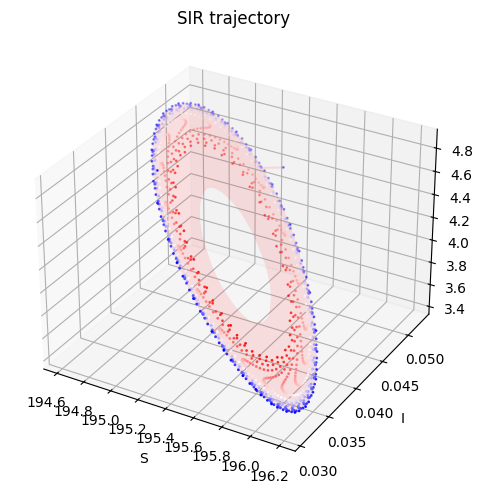
\includegraphics[width=0.3\textwidth]{images/t5_3-traj1.png}}
%\subfigure[$b=0.022$]{
%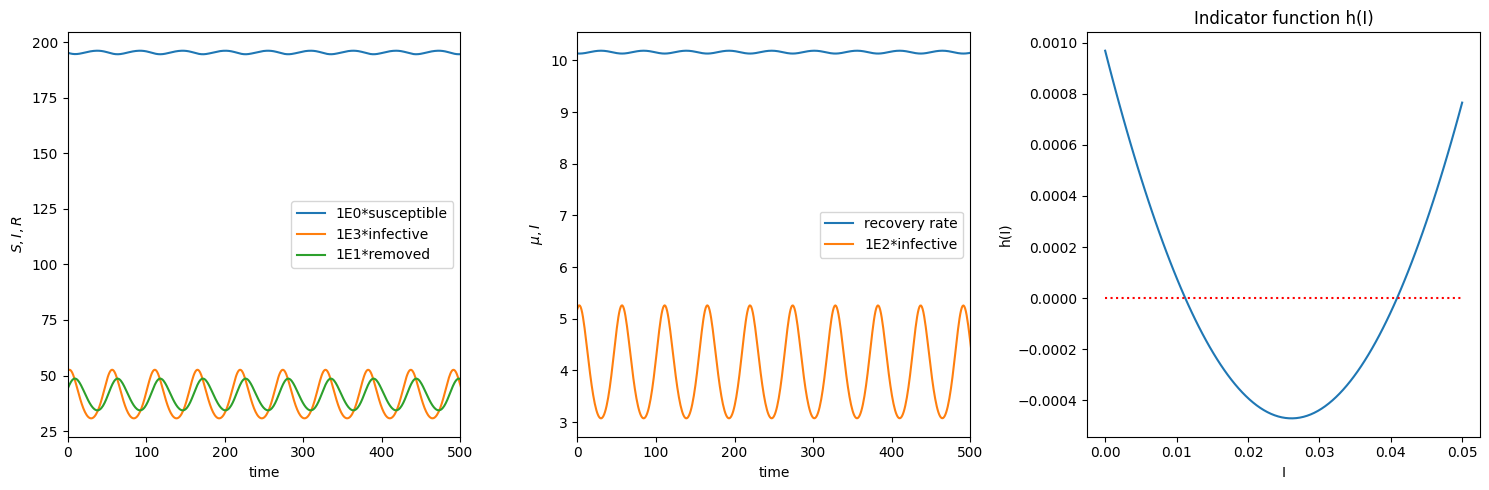
\includegraphics[width=0.6\textwidth]{images/t5_3-sim1.png}}
\subfigure[$b=0.024$]{
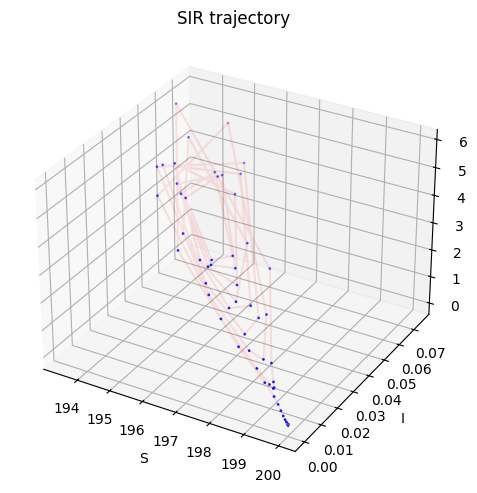
\includegraphics[width=0.3\textwidth]{images/t5_3-traj24.png}}
%\subfigure[$b=0.024$]{
%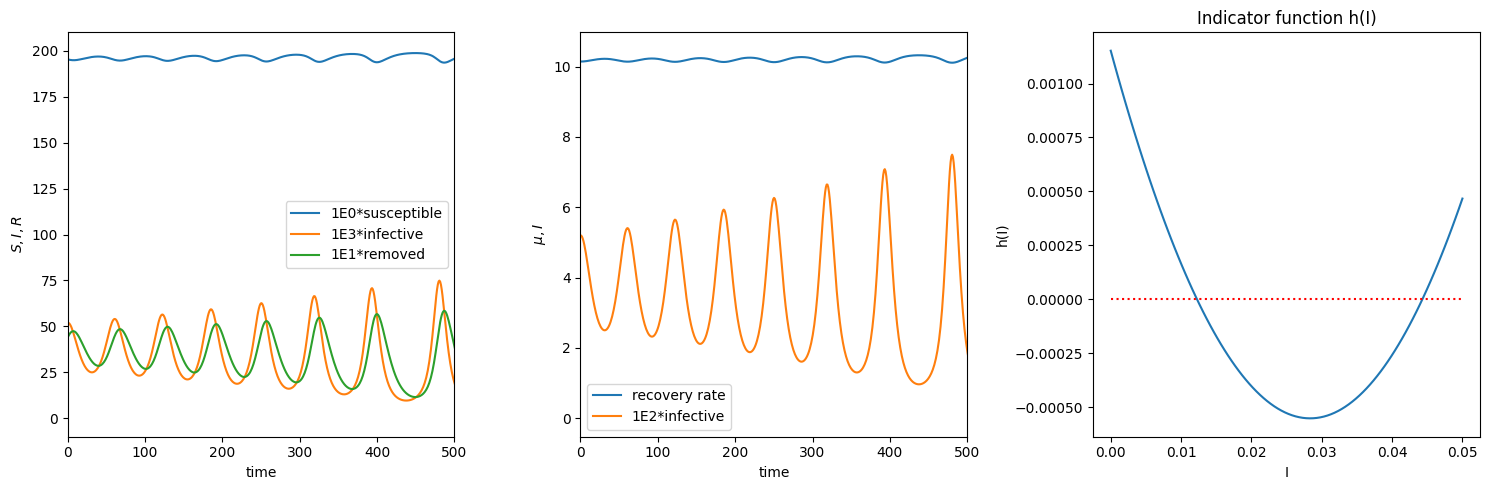
\includegraphics[width=0.6\textwidth]{images/t5_3-sim24.png}}
\subfigure[$b=0.022$]{
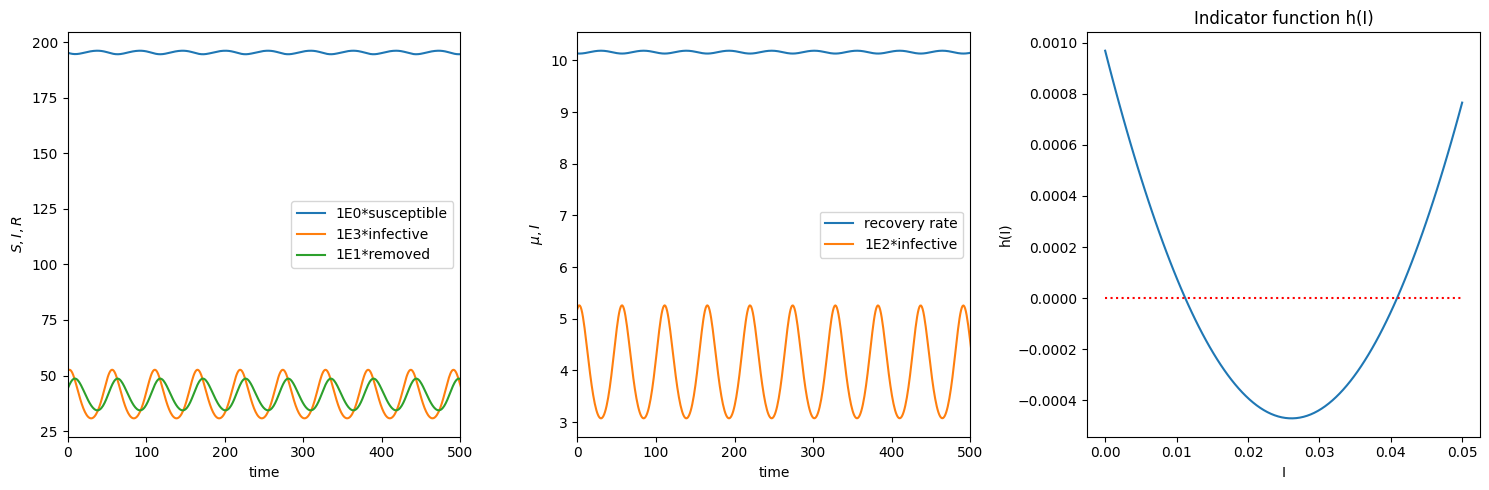
\includegraphics[width=0.9\textwidth]{images/t5_3-sim1.png}}
\caption{Plots for $(S_0, I_0, R_0 )=(195.3,0.052,4.4)$ and different $b$}
\label{fig:t5_3-trajB}
\end{figure}

\begin{figure}[H]
\centering
\subfigure[$(S_0, I_0, R_0 )=(195.7, 0.03, 3.92)$]{
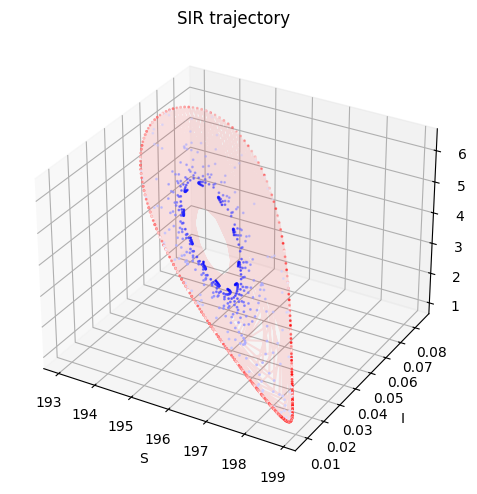
\includegraphics[width=0.3\textwidth]{images/t5_3-traj2.png}}
\subfigure[$(S_0, I_0, R_0 )=(193, 0.08, 6.21)$]{
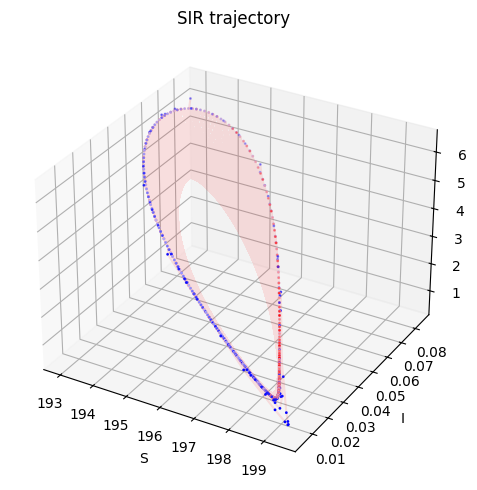
\includegraphics[width=0.3\textwidth]{images/t5_3-traj3.png}}
\caption{Plots for $b=0.022$ and other initial values $(S_0, I_0, R_0 )$}
\label{fig:t5_3-sims}
\end{figure}

\newpage
\paragraph{Task 5.4}
We observe the Hopf bifurcation at $b=0.022$. From the abstract of \cite{rosales2004hopf} "a Hopf bifurcations occurs as a spiral point switches from stable to unstable (or vice versa) and a periodic solution appears". In Figures \ref{fig:t5_3-trajB}(a) to (c) we see a spiral point switch from stable to unstable state. We see the periodic solution in first 2 figures of \ref{fig:t5_3-trajB}(d). But also from \cite{shan2014bifurcations} theorem 4.4 is proven i.e a generic Hopf bifurcation could occur. Then examples are provided as $(195.3, 0.052, 4.4)$ spirals inward to a stable focus (see \ref{fig:t5_3-trajB}(b)), $(195.3, 0.052, 4.4)$ spirals inward to the stable focus (see \ref{fig:t5_3-sims}(a)) and $(193, 0.08, 6.21)$ spirals inward to a stable limit cycle (see \ref{fig:t5_3-sims}(b)).

From \cite{Kuznetsov1998} page 84 the normal-form of the Hopf Bifurcation is defined as:
\begin{align*}
    \begin{cases}
        \dot{x}_1 = \alpha x_1 - x_2 - x_1 (x_1^2 + x_2^2),\\
        \dot{x}_2 = x_1 + \alpha x_2 - x_2 (x_1^2 + x_2^2)
    \end{cases}
\end{align*}

But as evidenced from testing with different parameters we observed that the dynamical system is dependant more than 2 parameters. Looking into \cite{shan2014bifurcations} section 4.3, it is also proven that the cusp type of Bogdanov–Takens bifurcation of codimension 3 occurs at $E_*$. In that section the prove of \cite{shan2014bifurcations} theorem 4.7 leads us to the normal-form:
\begin{align*}
    \begin{cases}
        \dot{X} &= Y,\\
        \dot{Y} &= \epsilon_1 + \epsilon_2 Y+\epsilon_3 XY+X^2 -X^3 Y+\mathcal{O}(|X,Y|^4)Y.
    \end{cases}
\end{align*}

Here $(\epsilon_1, \epsilon_2, \epsilon_3)$ are a function of the bifurcation parameters $(\mu_1, b, \beta)$.

\paragraph{Task 5.5}
From the implementation in \verb|sir_model.py| and \cite{shan2014bifurcations} we can draw the definition of the reproduction number $\mathbb{R}_0$. Here $\beta$ is the average number of adequate contacts per unit time with infectious individuals. $d$ is the per capita natural death rate. $\nu$ is the per capita disease-induced death rate. $\mu_1$ is the maximum recovery rates based on the number of available beds. The reproduction number is defined as the following:
\begin{align*}
    \mathbb{R}_0 = \frac{\beta}{d+\nu +\mu_1}
\end{align*}

Intuitively the reproduction rate $\mathbb{R}_0$ is the ratio between the average contacts with infected individuals per unit time and maximal rate of removing individuals. Essentially the reproduction rate $\mathbb{R}_0$ is the infection rate in relative to the (maximal) removal rate.

From \cite{van2002reproduction} section 3 the reproduction number $\mathbb{R}_0$ is cited as "the expected number of secondary cases produced, in a completely susceptible population, by a typical infective individual". Overall from \cite{van2002reproduction} we can conclude that, if $\beta$ increases or decreases the reproduction rate also increases or decreases. If the reproduction rate is $\mathbb{R}_0<1$, the infection can not grow. If $\mathbb{R}_0>1$ holds, then each infected individual produces more than one new infection on average and hence the infection can spread.

In our previous observations in Figure \ref{fig:t5_3-trajB} all reproduction numbers have been $\mathbb{R}_0 =0.99567 <1$. From \cite{shan2014bifurcations} Theorem 3.3 (4a) the implemented SIR model can have 2 endemic equilibria.

\paragraph{Task 5.6}
The plots for this task can be found in \verb|sir_bed_model-t5_6.ipynb|. We have $(S_0, I_0, R_0) = \mathbb{E}_0 = (A/d, 0,0)$ as initial values and it is obvious that all people become susceptible individuals. First off $S_0 = A/d$ where the count of the susceptible people is $A$ (recruitment/birth rate of susceptible population) divided by $d$ (per capita natural death rate). At the same time, we have no infected $I_0$ or removed $R_0$ individuals. Given this the initial state is disease free. Furthermore, the reproduction rate as defined in the previous section is $\mathbb{R}_0 <1$. Hence we know from \cite{van2002reproduction} section 3 that "on average an infected individual produces less than one new infected individual over the course of its infectious period, and the infection cannot grow".

Therefore the disease-free equilibrium $\mathbb{E}_0 = (A/d, 0,0)$ being an attracting node means that the trajectories in the dynamic system will move to this state. If we look at the figures in \ref{fig:t5_6-plots}(a), we observe all points gathered at the equilibrium $\mathbb{E}_0$ and given the initial values there are no infected and removed people in \ref{fig:t5_6-plots}(b).

Similarly, for $(S,I,R)$ values close to $\mathbb{E}_0$ we assume that all trajectories will lead to this disease-free equilibrium. When performing further testing for $(S,I,R)$ values close to $\mathbb{E}_0$ we can verify that all trajectories lead to the disease-free equilibrium as seen in Figure \ref{fig:t5_6-trajs}(a) to (c). But in Figure \ref{fig:t5_6-trajs}(d) to (f) we can also see that Hopf bifurcation can still occur given specific values. We can verify that $\beta > d+\nu+\mu_0$ holds in our simulations. We thus know from \cite{shan2014bifurcations} theorem 3.3 that $\mathbb{E}_0$ is not globally asymptotically stable, hence bifurcations seen in \ref{fig:t5_6-trajs}(d)-(f) are still possible.

\begin{figure}[H]
\centering
\subfigure[Trajectory of $\mathbb{E}_0$]{
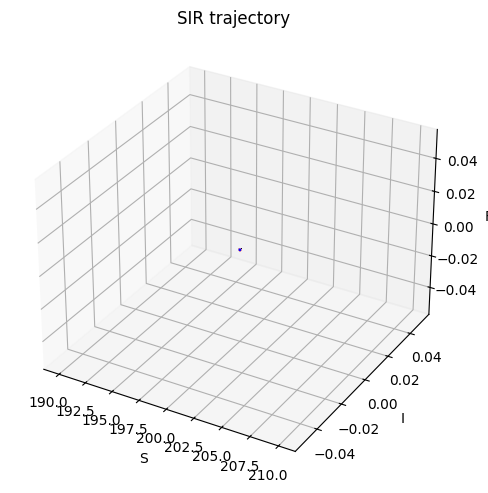
\includegraphics[width=0.3\textwidth]{images/t5_6-traj.png}}
\subfigure[Plots of $\mathbb{E}_0$]{
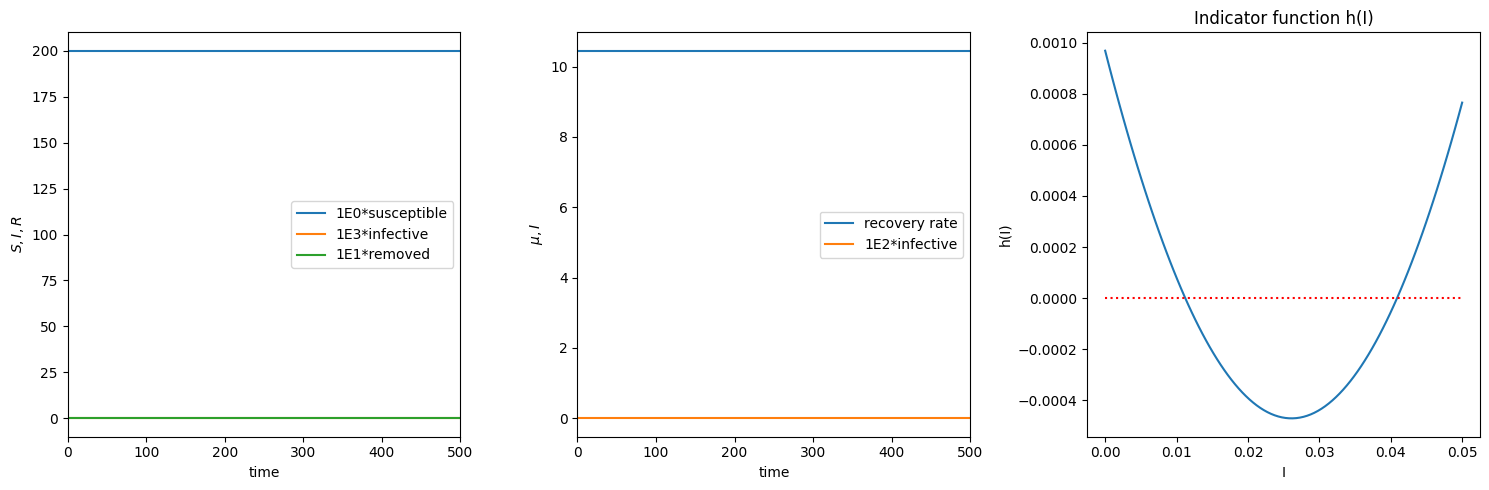
\includegraphics[width=0.6\textwidth]{images/t5_6-sim.png}}
\caption{Plots of disease-free equilibrium $\mathbb{E}_0=(A/d, 0,0)$}
\label{fig:t5_6-plots}
\end{figure}

\begin{figure}[H]
\centering
\subfigure[$(S_0, I_0, R_0) = (200, 0.5, 4.4)$]{
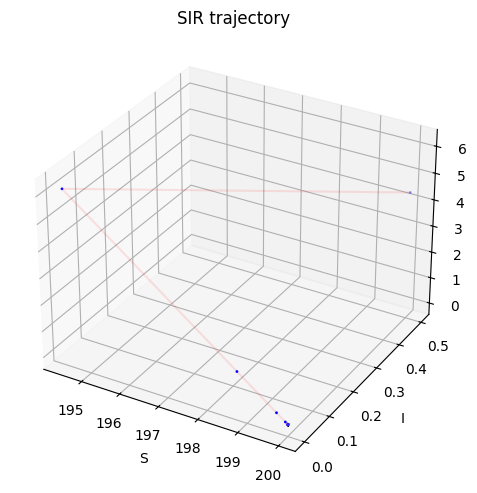
\includegraphics[width=0.3\textwidth]{images/t5_6-traj1.png}}
\subfigure[$(S_0, I_0, R_0) = (200, 0.05, 0.4)$]{
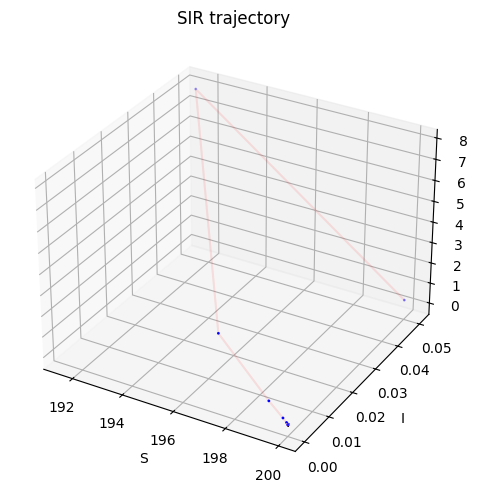
\includegraphics[width=0.3\textwidth]{images/t5_6-traj2.png}}
\subfigure[$(S_0, I_0, R_0) = (200, 0.5, 0.4)$]{
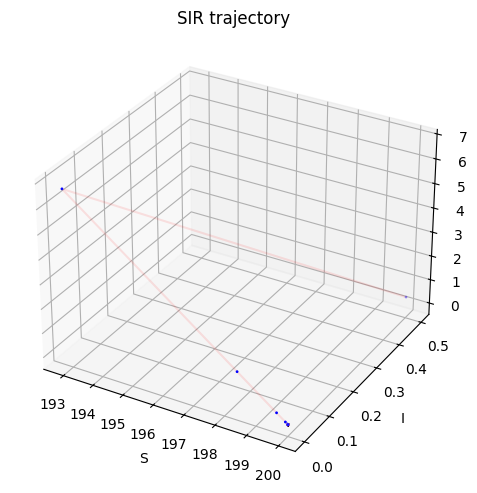
\includegraphics[width=0.3\textwidth]{images/t5_6-traj3.png}}
\subfigure[$(S_0, I_0, R_0) = (200, 0.052, 4.4)$]{
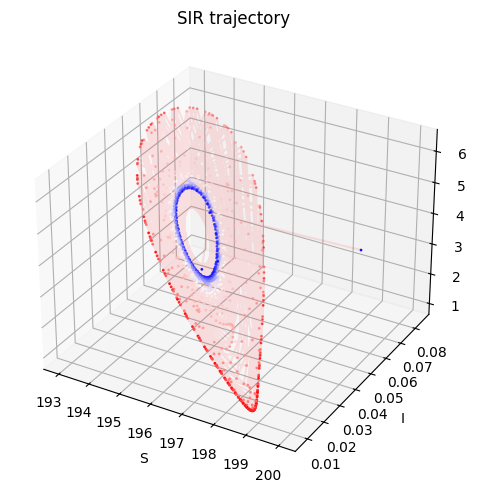
\includegraphics[width=0.3\textwidth]{images/t5_6-traj4.png}}
\subfigure[$(S_0, I_0, R_0) = (200, 0.050, 4.4)$]{
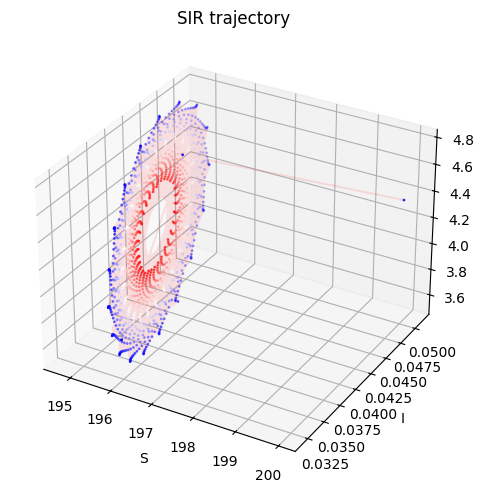
\includegraphics[width=0.3\textwidth]{images/t5_6-traj5.png}}
\subfigure[$(S_0, I_0, R_0) = (200, 0.052, 4.0)$]{
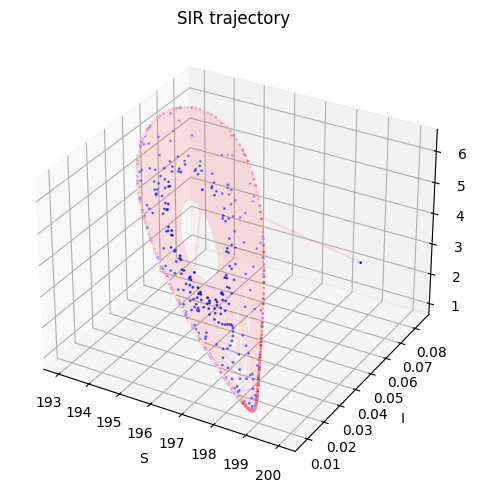
\includegraphics[width=0.3\textwidth]{images/t5_6-traj6.png}}
\caption{Trajectories of $b=0.022$ and $(S_0, I_0, R_0)$ close to $\mathbb{E}_0=(A/d, 0,0)$}
\label{fig:t5_6-trajs}
\end{figure}

\newpage
\paragraph{Task 5.7: Bonus}
For this task the code can be found in the python notebook \verb|sir_bed_model-t5_7.ipynb|. Before we start with the tests we can take note from section 4 Bifurcations in \cite{shan2014bifurcations}. It is shown that the SIR model from \cite{shan2014bifurcations} can undergo the multiple kinds of bifurcations such as:
\begin{itemize}
    \item Forward bifurcation
    \item Backward bifurcation
    \item Pitchfork bifurcation
    \item Saddle-node bifurcation
    \item Hopf bifurcation
    \item Cusp type of Bogdanov–Takens bifurcation
\end{itemize}

 We have previously visualized Hopf bifurcation and in the following we will try to replicate a pitchfork bifurcation. As stated in \cite{shan2014bifurcations} Theorem (4.1) we are considering $\mathbb{R}_0$ as bifurcation parameter. The proof below the theorem  further states that due to the definition of $\mathbb{R}_0$ we can use $\mu_1$ as bifurcation parameter without loss of generality. Then the necessary conditions for a pitchfork bifurcation to occur are namely the following:

\begin{align*}
    \mu_1 &= \beta -d-\nu+\epsilon\\
    b_{pitchfork}:=b &= \frac{A(\mu_1 -\mu_0)}{\beta (\beta -\nu)}\\
\end{align*}

For better comparison we also decided to additionally visualize forward and backward bifurcations. According to theorem 4.1 (1) these are respectively obtained when
$b > \frac{A(\mu_1 -mu_0)}{\beta (\beta -\nu)}$ and $b < \frac{A(\mu_1 -mu_0)}{\beta (\beta -\nu)}$ holds. All parameters are set as given for task 5.3 with exception of the following. In previous iterations of the notebook the initial values $(S_0, I_0, R_0)$ have led to interesting plots, hence these initial values will be used across all experiments. Since $b$ can be chosen arbitrarily we have decided to use similar values as in the paper \cite{shan2014bifurcations} Figure 7 (a) and (b), so that we can potentially obtain similar plots as in the paper. These use $b=0.07$ for forward bifurcation and $b=0.04$ for backward bifurcation.\\

In figures \ref{fig:t5_7-traj}(d)(e)(f) we see their trajectories of each bifurcation when plotting in 3d. Since $R$ axis is not relevant it is easier to analyse the trajectories in the $(S,I)$ plane. This can be seen in \ref{fig:t5_7-traj}(a)(b)(c). Note that the color gradient describes the change of the $(S,I,R)$ values over time $t$. Here $t=0$ is blue and turns white and then into red when reaching the end $t=t_{max}$.

Figure \ref{fig:t5_7-traj}(a) and (d) are the trajectories of the pitchfork bifurcation and unfortunately it is very hard to interpret it. But if we look at the trajectories of the forward (Fig. \ref{fig:t5_7-traj}(b)(e)) and backward bifurcation (Fig. \ref{fig:t5_7-traj}(c)(f)) we can see their similarities as well as their polar behaviour. The opposite development of their trajectories can be simply explained from their relation to the variable $b$. For \ref{fig:t5_7-traj}(b) we could form a correlation that the amount of hospital beds $b>b_{pitchfork}$ leads to a decrease of infected over time (indicated by the coloring) given that the reproduction number is fixed as $\mathbb{R}_0=1$. Similarly observed in \ref{fig:t5_7-traj}(c) $b>b_{pitchfork}$ In infected show an increase behaviour over time. When observing \ref{fig:t5_7-traj}(b)(c) from the perspective of $S$, we observe periodic behaviour. This probably captures the constant, but fluctuating behaviour of the birthrate for $S$. Additionally we can speculate the the existence of this periodic behaviour is what causes Hopf bifurcations.

Combining previous observations we can assume that the pitchfork bifurcation in \ref{fig:t5_7-traj}(a) is the point between forward and backward bifurcation, when it comes to their trajectories. This is further more expanded when observing their trajectories in 3d \ref{fig:t5_7-traj}(d)-(f). We can confirm this behaviour when checking \cite{shan2014bifurcations} Figure 2, where the point $K$ lies between the sets of values $C^+_0$ and $C^-_0$, which represent the $(\mu_1,b)$ tuples when forward and backward bifurcations occur.

\begin{figure}[H]
\centering
\subfigure[Trajectory of Pitchfork Bifurcation]{
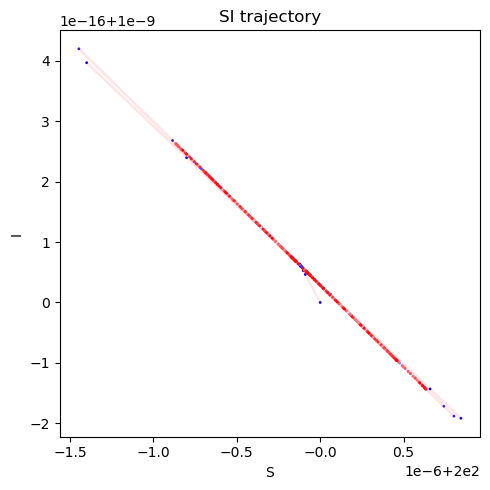
\includegraphics[width=0.3\textwidth]{images/t5_7-pf-traj.png}}
\subfigure[Trajectory of Forward Bifurcation]{
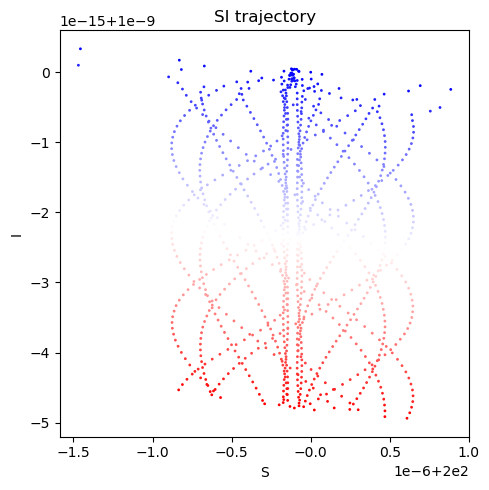
\includegraphics[width=0.3\textwidth]{images/t5_7-fw-traj.png}}
\subfigure[Trajectory of Backward Bifurcation]{
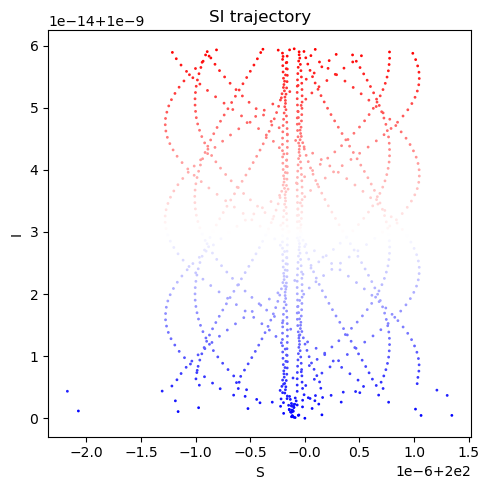
\includegraphics[width=0.3\textwidth]{images/t5_7-bw-traj.png}}
\subfigure[Trajectory of Pitchfork Bifurcation]{
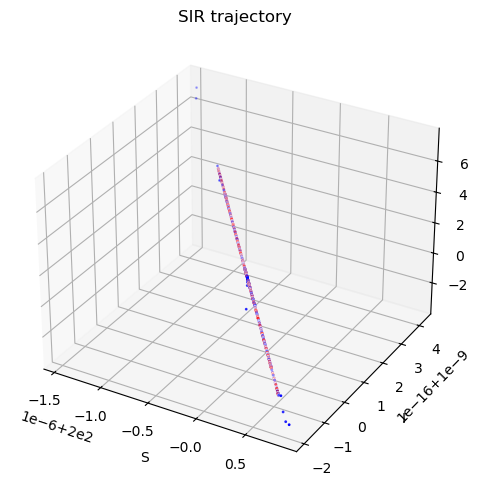
\includegraphics[width=0.3\textwidth]{images/t5_7-pf-traj3d.png}}
\subfigure[Trajectory of Forward Bifurcation]{
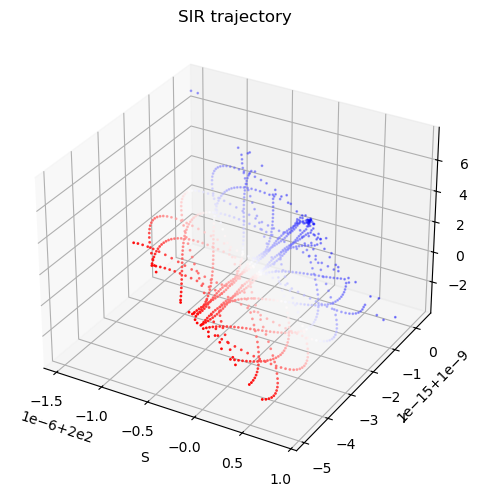
\includegraphics[width=0.3\textwidth]{images/t5_7-fw-traj3d.png}}
\subfigure[Trajectory of Backward Bifurcation]{
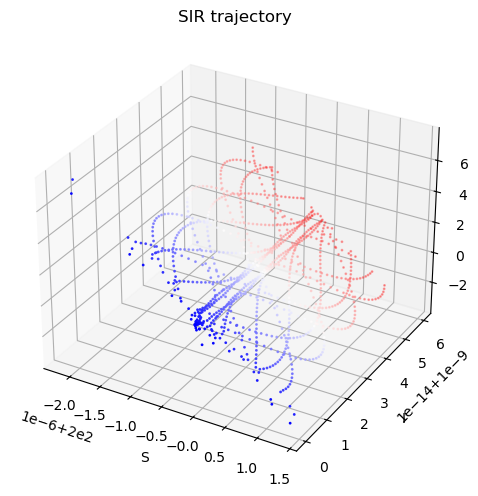
\includegraphics[width=0.3\textwidth]{images/t5_7-bw-traj3d.png}}
\caption{Trajectories in $S,I$ and $S,I,R$ plane}
\label{fig:t5_7-traj}
\end{figure}

Since the trajectories can not paint the full picture, we will next look at their bifurcation diagrams. This idea is inspired by \cite{shan2014bifurcations} Figure 7, since reproducing similar diagrams would confirm that we have plotted the pitchfork bifurcation correctly. In figures \ref{fig:t5_7-R0}(a)(b)(c) the reproduction number $\mathbb{R}_0$ is plotted against $I$. Note that $\mathbb{R}_0$ is treated as bifurcation parameter, but the implementation only change $\mu_1$, affecting $\mathbb{R}_0$ in consequence. Since $\mu_1$ is the bifurcation parameter we need to recalculate the number of infected $I$ every time.

For better understanding of plotting $\mathbb{R}_0$ against $I$ we also plotted it in 3d against $t$ in figures \ref{fig:t5_7-R0}(d)(e)(f). When excluding small $t$-values we can confirm that bifurcation diagram is consistent across all time slices.\\

The initial observation is that all bifurcation diagrams look similar. We can easily confirm that \ref{fig:t5_7-R0}(b) is behaving as expected, when comparing it to \cite{shan2014bifurcations} Figure 7(a). In a forward bifurcation, as the bifurcation parameter crosses a critical threshold, the system transitions from one stable state to another. Before the threshold we are in the disease-free equilibrium and afterwards the onset of the epidemic is seen as $\mathbb{R}_0$ crosses the threshold of 1.

As for backward bifurcation Figure 7(b) from \cite{shan2014bifurcations} shows that the existence of an epidemic extends also for some values below $\mathbb{R}_0<1$. While \ref{fig:t5_7-R0} does not fully capture this (due to implementations haven taken too long up to this point), we can see that the cut-off at $\mathbb{R}=1$ implies this behaviour of the backwards bifurcation.

When looking at \ref{fig:t5_7-R0}(a) we can not that the bifurcation diagram is likely the same as the forward bifurcation. We can say at this point that like the forward bifurcation, the pitchfork bifurcation marks the start of an epidemic as well, when crossing $\mathbb{R}_0$. Unfortunately the pitchfork bifurcation does not show the characteristic pitchfork shape. Logically speaking it wouldn't make sense to observe a decrease in infected individuals given that there is none, while increasing the reproduction number crossing the threshold $\mathbb{R}_0 = 1$. Looking back into \cite{shan2014bifurcations} the proof of theorem 4.1 shows that the set of points describing pitchfork bifurcations can be described using the following:

\begin{align*}
    C^\pm_{\Delta}: b&=f^\pm_{\Delta}(\mu_1)\triangleq\frac{\beta (\mu_1-\mu_0)+\delta_0(\delta_1-\beta)\pm \sqrt{\beta\delta_1(\mu_1-\mu_0)(\delta_1-\beta)}}{(\beta-\nu)\delta_1^2}\\
    \delta_0 &= d+\nu+\mu_0\\
    \delta_1 &= d+\nu+\mu_1
\end{align*}

It can then be verified that then $f^\pm_{\Delta}(\delta-d-\nu)=\frac{A(\mu1-\mu0)}{\beta()\beta-\nu}$ holds. This is verified in the python notebook as well using the functions \verb|f_plus(...)| and \verb|f_minus(...)|. This explains why the pitchfork bifurcation in $\mathbb{R}_0,I$ plane shows the same behaviour as the forward bifurcation. The observe characteristic we would probably instead need to plot $b$ against $\mu_1$ using the definition $b=f^\pm_{\Delta}(\mu_1)$. The curves of $C_0^+$ and $C^-_0$ could be interpreted as the pitchfork.\\

Overall we can see that SIR model described using the differential equations in \cite{shan2014bifurcations}(2.2) is a very complex dynamical system. In this task have observed that different bifurcations can occur given the right settings. As for the pitchfork bifurcation it exists under special conditions such that the forking part overlaps with each other.

\begin{figure}[H]
\centering
\subfigure[Pitchfork Bifurcation at $t=999$]{
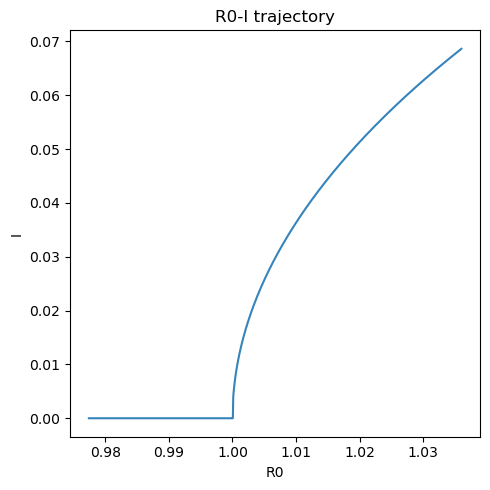
\includegraphics[width=0.3\textwidth]{images/t5_7-pf-R0.png}}
\subfigure[Forward Bifurcation at $t=999$]{
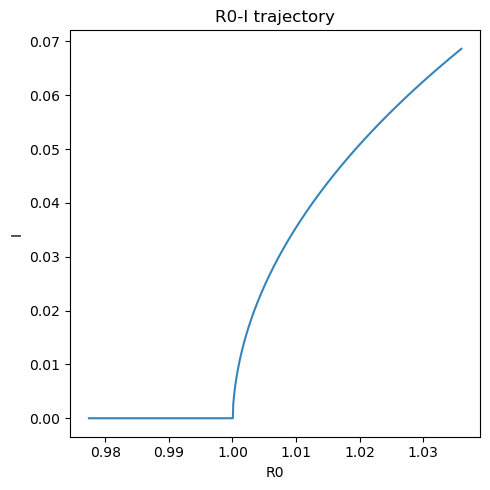
\includegraphics[width=0.3\textwidth]{images/t5_7-fw-R0.png}}
\subfigure[Backward Bifurcation at $t=999$]{
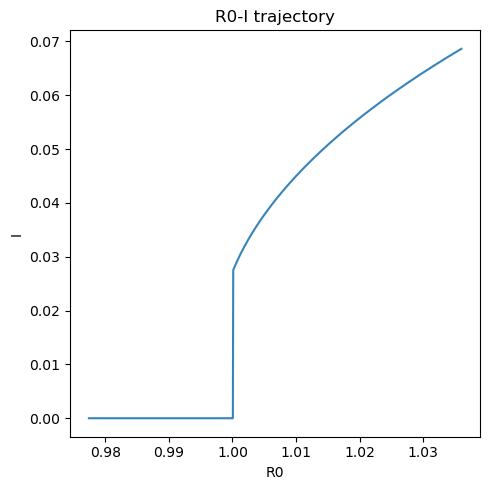
\includegraphics[width=0.3\textwidth]{images/t5_7-bw-R0.png}}
\subfigure[3D plot of Pitchfork Bifurcation]{
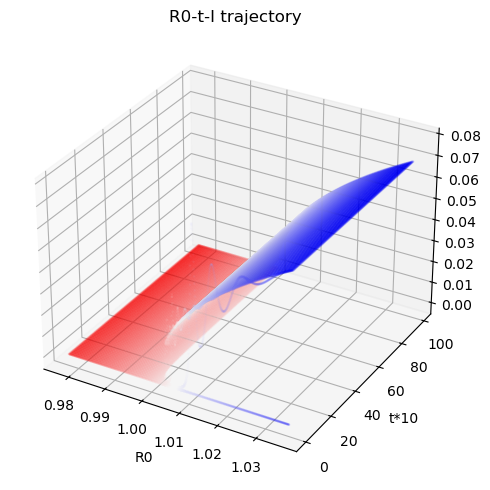
\includegraphics[width=0.3\textwidth]{images/t5_7-pf-R03d.png}}
\subfigure[3D plot of Forward Bifurcation]{
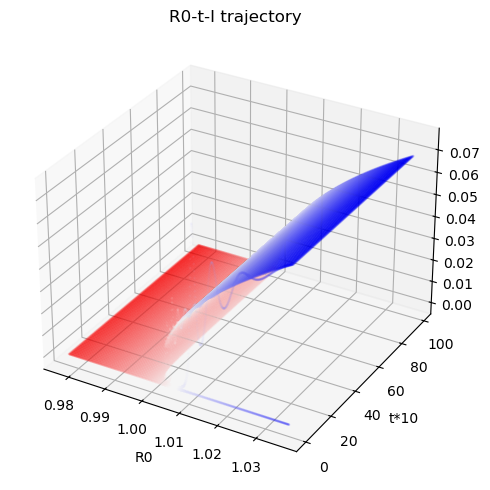
\includegraphics[width=0.3\textwidth]{images/t5_7-fw-R03d.png}}
\subfigure[3D plot of Backward Bifurcation]{
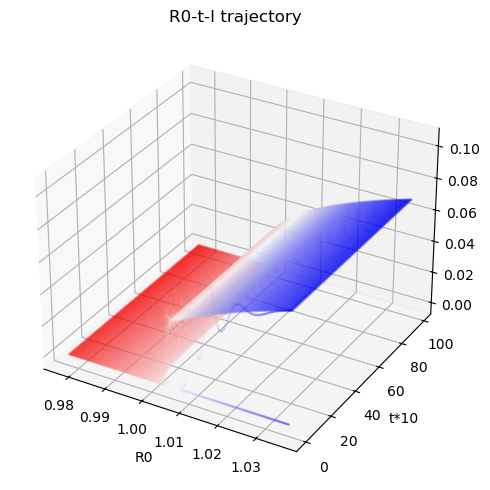
\includegraphics[width=0.3\textwidth]{images/t5_7-bw-R03d.png}}
\caption{Bifurcation diagram on $\mathbb{R}_0, I$ plane}
\label{fig:t5_7-R0}
\end{figure}

\end{task}

\bibliographystyle{plain}
\bibliography{Literature}

\end{document}